\documentclass[12pt]{article}
%DIF LATEXDIFF DIFFERENCE FILE


\usepackage[top=1in,left=1in, right = 1in, footskip=1in]{geometry}

\usepackage{graphicx}
%\usepackage{adjustbox}

\newcommand{\eref}[1]{(\ref{eq:#1})}
\newcommand{\fref}[1]{Fig.~\ref{fig:#1}}
\newcommand{\Fref}[1]{Fig.~\ref{fig:#1}}
\newcommand{\sref}[1]{Sec.~\ref{#1}}
\newcommand{\frange}[2]{Fig.~\ref{fig:#1}--\ref{fig:#2}}
\newcommand{\tref}[1]{Table~\ref{tab:#1}}
\newcommand{\tlab}[1]{\label{tab:#1}}
\newcommand{\seminar}{SE\mbox{$^m$}I\mbox{$^n$}R}

\usepackage{amsthm}
\usepackage{amsmath}
\usepackage{amssymb}
\usepackage{amsfonts}

\usepackage{lineno}
%\linenumbers

\usepackage[pdfencoding=auto, psdextra]{hyperref}

\bibliographystyle{chicago}
\usepackage{natbib}
\date{\today}

\usepackage{xspace}
\newcommand*{\ie}{i.e.\@\xspace}

\usepackage{color}

\newcommand{\Rx}[1]{\ensuremath{{\mathcal R}_{#1}}} 
\newcommand{\Ro}{\Rx{0}}
\newcommand{\RR}{\ensuremath{{\mathcal R}}}
\newcommand{\Rhat}{\ensuremath{{\hat\RR}}}
\newcommand{\tsub}[2]{#1_{{\textrm{\tiny #2}}}}

\newcommand{\comment}[3]{\textcolor{#1}{\textbf{[#2: }\textsl{#3}\textbf{]}}}
\newcommand{\jd}[1]{\comment{cyan}{JD}{#1}}
\newcommand{\swp}[1]{\comment{magenta}{SWP}{#1}}
\newcommand{\dc}[1]{\comment{blue}{DC}{#1}}
\newcommand{\hotcomment}[1]{\comment{red}{HOT}{#1}}

\newcommand{\jdnew}{\jd{NEW}}
\newcommand{\jddel}[1]{\jd{DELETE: #1}}
%DIF PREAMBLE EXTENSION ADDED BY LATEXDIFF
%DIF UNDERLINE PREAMBLE %DIF PREAMBLE
\RequirePackage[normalem]{ulem} %DIF PREAMBLE
\RequirePackage{color}\definecolor{RED}{rgb}{1,0,0}\definecolor{BLUE}{rgb}{0,0,1} %DIF PREAMBLE
\providecommand{\DIFaddtex}[1]{{\protect\color{blue}\uwave{#1}}} %DIF PREAMBLE
\providecommand{\DIFdeltex}[1]{{\protect\color{red}\sout{#1}}}                      %DIF PREAMBLE
%DIF SAFE PREAMBLE %DIF PREAMBLE
\providecommand{\DIFaddbegin}{} %DIF PREAMBLE
\providecommand{\DIFaddend}{} %DIF PREAMBLE
\providecommand{\DIFdelbegin}{} %DIF PREAMBLE
\providecommand{\DIFdelend}{} %DIF PREAMBLE
\providecommand{\DIFmodbegin}{} %DIF PREAMBLE
\providecommand{\DIFmodend}{} %DIF PREAMBLE
%DIF FLOATSAFE PREAMBLE %DIF PREAMBLE
\providecommand{\DIFaddFL}[1]{\DIFadd{#1}} %DIF PREAMBLE
\providecommand{\DIFdelFL}[1]{\DIFdel{#1}} %DIF PREAMBLE
\providecommand{\DIFaddbeginFL}{} %DIF PREAMBLE
\providecommand{\DIFaddendFL}{} %DIF PREAMBLE
\providecommand{\DIFdelbeginFL}{} %DIF PREAMBLE
\providecommand{\DIFdelendFL}{} %DIF PREAMBLE
%DIF HYPERREF PREAMBLE %DIF PREAMBLE
\providecommand{\DIFadd}[1]{\texorpdfstring{\DIFaddtex{#1}}{#1}} %DIF PREAMBLE
\providecommand{\DIFdel}[1]{\texorpdfstring{\DIFdeltex{#1}}{}} %DIF PREAMBLE
\newcommand{\DIFscaledelfig}{0.5}
%DIF HIGHLIGHTGRAPHICS PREAMBLE %DIF PREAMBLE
\RequirePackage{settobox} %DIF PREAMBLE
\RequirePackage{letltxmacro} %DIF PREAMBLE
\newsavebox{\DIFdelgraphicsbox} %DIF PREAMBLE
\newlength{\DIFdelgraphicswidth} %DIF PREAMBLE
\newlength{\DIFdelgraphicsheight} %DIF PREAMBLE
% store original definition of \includegraphics %DIF PREAMBLE
\LetLtxMacro{\DIFOincludegraphics}{\includegraphics} %DIF PREAMBLE
\newcommand{\DIFaddincludegraphics}[2][]{{\color{blue}\fbox{\DIFOincludegraphics[#1]{#2}}}} %DIF PREAMBLE
\newcommand{\DIFdelincludegraphics}[2][]{% %DIF PREAMBLE
\sbox{\DIFdelgraphicsbox}{\DIFOincludegraphics[#1]{#2}}% %DIF PREAMBLE
\settoboxwidth{\DIFdelgraphicswidth}{\DIFdelgraphicsbox} %DIF PREAMBLE
\settoboxtotalheight{\DIFdelgraphicsheight}{\DIFdelgraphicsbox} %DIF PREAMBLE
\scalebox{\DIFscaledelfig}{% %DIF PREAMBLE
\parbox[b]{\DIFdelgraphicswidth}{\usebox{\DIFdelgraphicsbox}\\[-\baselineskip] \rule{\DIFdelgraphicswidth}{0em}}\llap{\resizebox{\DIFdelgraphicswidth}{\DIFdelgraphicsheight}{% %DIF PREAMBLE
\setlength{\unitlength}{\DIFdelgraphicswidth}% %DIF PREAMBLE
\begin{picture}(1,1)% %DIF PREAMBLE
\thicklines\linethickness{2pt} %DIF PREAMBLE
{\color[rgb]{1,0,0}\put(0,0){\framebox(1,1){}}}% %DIF PREAMBLE
{\color[rgb]{1,0,0}\put(0,0){\line( 1,1){1}}}% %DIF PREAMBLE
{\color[rgb]{1,0,0}\put(0,1){\line(1,-1){1}}}% %DIF PREAMBLE
\end{picture}% %DIF PREAMBLE
}\hspace*{3pt}}} %DIF PREAMBLE
} %DIF PREAMBLE
\LetLtxMacro{\DIFOaddbegin}{\DIFaddbegin} %DIF PREAMBLE
\LetLtxMacro{\DIFOaddend}{\DIFaddend} %DIF PREAMBLE
\LetLtxMacro{\DIFOdelbegin}{\DIFdelbegin} %DIF PREAMBLE
\LetLtxMacro{\DIFOdelend}{\DIFdelend} %DIF PREAMBLE
\DeclareRobustCommand{\DIFaddbegin}{\DIFOaddbegin \let\includegraphics\DIFaddincludegraphics} %DIF PREAMBLE
\DeclareRobustCommand{\DIFaddend}{\DIFOaddend \let\includegraphics\DIFOincludegraphics} %DIF PREAMBLE
\DeclareRobustCommand{\DIFdelbegin}{\DIFOdelbegin \let\includegraphics\DIFdelincludegraphics} %DIF PREAMBLE
\DeclareRobustCommand{\DIFdelend}{\DIFOaddend \let\includegraphics\DIFOincludegraphics} %DIF PREAMBLE
\LetLtxMacro{\DIFOaddbeginFL}{\DIFaddbeginFL} %DIF PREAMBLE
\LetLtxMacro{\DIFOaddendFL}{\DIFaddendFL} %DIF PREAMBLE
\LetLtxMacro{\DIFOdelbeginFL}{\DIFdelbeginFL} %DIF PREAMBLE
\LetLtxMacro{\DIFOdelendFL}{\DIFdelendFL} %DIF PREAMBLE
\DeclareRobustCommand{\DIFaddbeginFL}{\DIFOaddbeginFL \let\includegraphics\DIFaddincludegraphics} %DIF PREAMBLE
\DeclareRobustCommand{\DIFaddendFL}{\DIFOaddendFL \let\includegraphics\DIFOincludegraphics} %DIF PREAMBLE
\DeclareRobustCommand{\DIFdelbeginFL}{\DIFOdelbeginFL \let\includegraphics\DIFdelincludegraphics} %DIF PREAMBLE
\DeclareRobustCommand{\DIFdelendFL}{\DIFOaddendFL \let\includegraphics\DIFOincludegraphics} %DIF PREAMBLE
%DIF END PREAMBLE EXTENSION ADDED BY LATEXDIFF

\begin{document}

\begin{flushleft}{
	\Large
	\textbf\newline{
		Modeling the population-level impact of a third dose of MMR vaccine on a mumps outbreak at the University of Iowa
	}
}
\newline
Sang Woo Park\textsuperscript{1},
Tomi Lawal\textsuperscript{2},
Mona Marin\textsuperscript{3},
Mariel A. Marlow\textsuperscript{3},
Bryan T. Grenfell\textsuperscript{1},
Nina B. Masters\textsuperscript{3}
\\ 
\bigskip
\textbf{1} Department of Ecology and Evolutionary Biology, Princeton University, Princeton, NJ, USA
\\
\textbf{2} University of Michigan Medical School, Ann Arbor, MI, USA
\\
\textbf{3} Division of Viral Diseases, Centers for Disease Control and Prevention, Atlanta, GA, USA
\end{flushleft} 

\section*{Abstract}

Mumps outbreaks among fully vaccinated young adults have raised questions about potential waning of immunity over time and need for a third dose of the measles, mumps, rubella (MMR) vaccine. 
However, there are currently limited data on real-life effectiveness of the third dose MMR vaccine in preventing mumps.
Here, we used a deterministic compartmental model to infer the effectiveness of the third dose MMR vaccine in preventing mumps cases by analyzing the mumps outbreak that occurred at the University of Iowa between August 24, 2015 and May 13, 2016. 
The modeling approach further allowed us to evaluate the population-level impact of vaccination by different timings of vaccine administration in relation to the beginning of the outbreak and different coverage levels and to account for potential sources of biases in estimating vaccine effectiveness. 
We found large uncertainty in vaccine effectiveness estimates: school holidays, such as the winter break, likely played important roles in preventing mumps transmission. 
Early introduction of a third vaccine dose during a mumps outbreak can be effective in preventing transmission. 
\\
\newline
\textbf{Disclaimer.} The findings and conclusions in this report are those of the authors and do not necessarily represent the official position of the Centers for Disease Control and Prevention.

\section*{Significance}
The resurgence of mumps among vaccinated young adults in the US continues to raise questions about the need for a third dose of the MMR vaccine, but existing estimates of third-dose vaccine effectiveness are limited.
We analyzed a mumps outbreak that occurred at the University of Iowa using a mathematical modeling approach which allowed us to account for different sources of biases. 
We estimate that while vaccination played a role in improving protection of persons at increased risk and preventing transmission during the outbreak, its overall impact on outbreak control was uncertain. 
However, school holidays likely had the greatest impact on preventing mumps transmission. 
Our analysis further highlights the importance of early introduction of vaccination in preventing outbreaks.

\section*{Keywords}
Mumps, MMR3, vaccine effectiveness, mathematical modeling, Bayesian inference

\pagebreak

\section{Introduction}

Mumps is an acute, vaccine-preventable viral disease, which typically presents with the swelling of the salivary parotid gland \citep{hviid2008mumps}.
It is transmitted by respiratory or salivary droplets.
Before introduction of vaccination, peak incidence was among children aged 5–9 years \citep{galazka1999mumps}.
Since the introduction of the mumps vaccine in 1967 nationwide in the United States (U.S.)---followed by the recommendation for routine second dose of the measles, mumps, rubella (MMR) vaccine in 1989 for measles prevention---U.S. mumps cases decreased by more than 99\% by early 2000s \citep{mclean2013prevention}.
However, cases and outbreaks have resurged in the U.S. \citep{ogbuanu2012impact,nelson2013epidemiology,cardemil2017effectiveness,wohl2020combining,lo2021influenza} and other industrialized countries since mid-2000s, particularly among young adults despite high vaccination rates \citep{aasheim2014outbreak,vygen2016waning}.
Mumps resurgence among highly vaccinated populations has been postulated to be caused by lower levels of vaccine-induced antibodies against the circulating wild-type genotype G virus strains compared with the live-attenuated vaccine genotype A virus strain (antigenic mismatch) \citep{peltola2007mumps,rubin2008antibody}, or from decreased immunity over time following vaccination (waning immunity) \citep{lewnard2018vaccine,seagle2018measles,gokhale2023disentangling}, both of which may reduce vaccine effectiveness (VE).

The resurgence of mumps outbreaks has raised questions about the need for third dose of the MMR vaccine.
In a review of the evidence, the Advisory Committee on Immunization Practices \citep{marin2018recommendation} identified three studies that reported lower attack rates among third dose MMR (MMR3) recipients compared to two-dose (MMR2) recipients during ongoing outbreaks \citep{ogbuanu2012impact,nelson2013epidemiology,cardemil2017effectiveness}, but only one found a statistically significant difference \citep{cardemil2017effectiveness}. 
Several studies reported significant increases in mumps antibody levels one month after MMR3 with decrease at one year \citep{fiebelkorn2014mumps,latner2017mumps,kaaijk2020third};
in addition, Kaaijk et al. reported that the antibody levels at one year were still higher than the baseline, suggesting a potential longer benefit than previously assumed. 
However, data on the effectiveness of the third dose MMR, including over time, remains limited.

Based on a mumps outbreak at the University of Iowa, \cite{cardemil2017effectiveness} previously estimated that students who had received three doses of MMR vaccine were at 78.1\% (95\% CI: 60.9\%--87.8\%) lower risk of mumps 28 days after vaccination than those who had received two doses.
However, this estimate did not consider the differences in forces of infection between the two groups, the effect of school holidays in preventing transmission, or the effectiveness of the third dose in preventing infection. 

In this study, we analyzed the mumps outbreak at the University of Iowa to infer the effectiveness of the third dose of MMR vaccine in preventing mumps using a deterministic mathematical model that allowed us to also characterize patterns of spread, evaluate the population-level impact of vaccination by timing of vaccine administration and coverage, and tease apart the impact of vaccination and school holidays.

\section{Methods}

\subsection{Data}

We analyzed a daily time series of mumps cases and the numbers of MMR vaccine doses administered during the University of Iowa mumps outbreak, August 24, 2015--May 13, 2016 (\fref{data}).
The University of Iowa had an undergraduate population of 20,496 during the 2015--2016 academic year and a mandatory two-dose MMR vaccine policy in place since 2012 with few exemptions.
Ninety-eight percent of students between 18--24 years of age had received at least two doses of MMR vaccine before the outbreak (1.8\% had received 3 doses and 0.1\% had received 4 dosese of MMR before the outbreak) \citep{cardemil2017effectiveness}.
Mumps cases were classified according to the Council of State and Territorial Epidemiologists case definition \citep{casedef}. 
The MMR vaccination campaign during the outbreak targeted students under 25 years through 8 free vaccination clinics, held from November 10--19, 2015. 
Overall, 259 mumps cases were identified and 4790 MMR vaccine doses were administered, of which 97\% were deemed to be third doses \citep{cardemil2017effectiveness}.
The student data used for this analysis (and also by \cite{cardemil2017effectiveness}) were restricted to those aged 18 to 24 years by the start of the first clinic. 

We also considered four major school holidays, which could have affected transmission dynamics during the outbreak (\fref{data}; \cite{iowa}): 
Thanksgiving break (November 22--29, 2015), winter break (December 11--28, 2015), between-term break (January 15--19, 2016), and spring break (March 13--20, 2016).
Classes were either recessed or closed during these periods, meaning that contact rates between students likely decreased, reducing transmission.

\begin{figure}[!th]
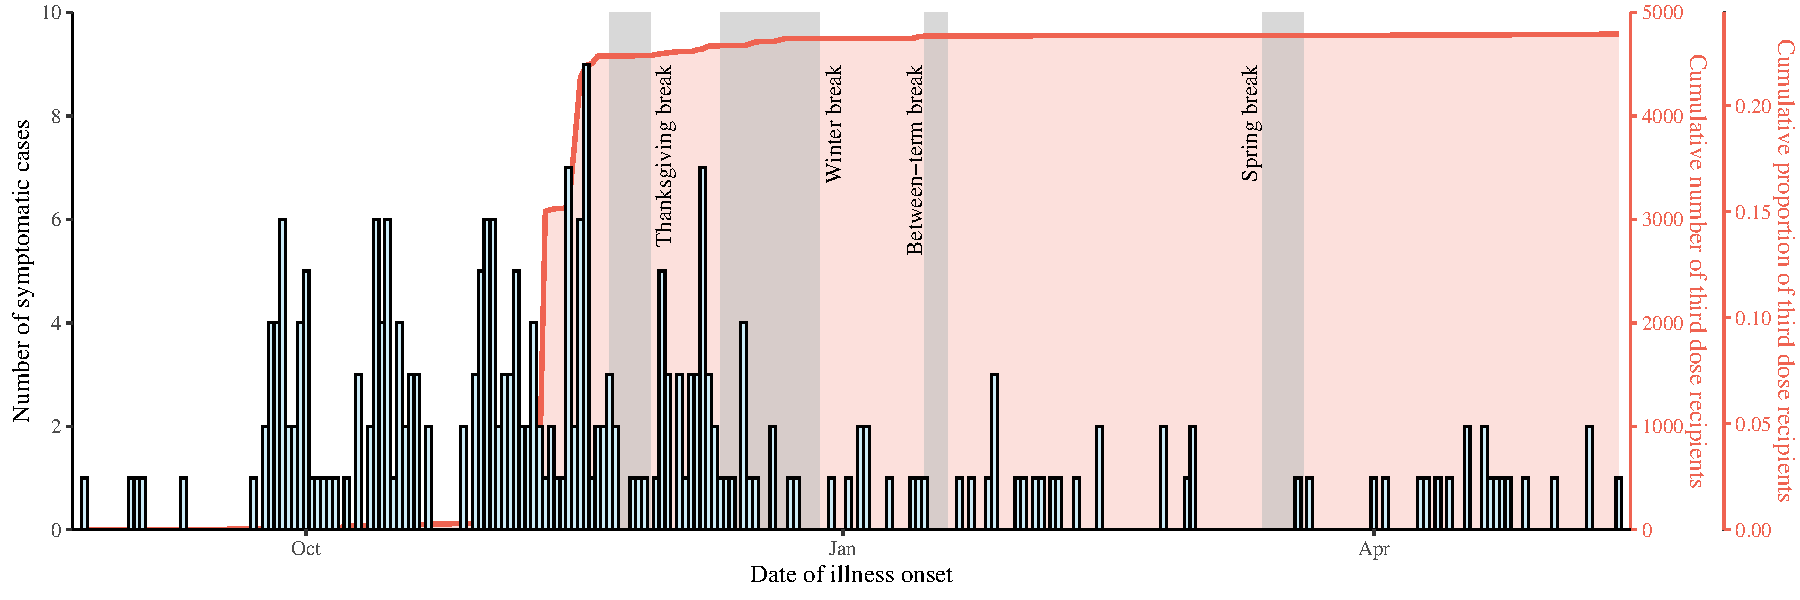
\includegraphics[width=\textwidth]{../figure/time_series.pdf}
\caption{
\textbf{Time series of mumps outbreak at the University of Iowa.}
Epidemic curve representing the number of students who developed symptoms on each day.
Gray shaded regions represent school breaks: Thanksgiving break (November 22--29, 2015), winter break (December 11--28, 2015), between-term break (January 15--19, 2016), and spring break (March 13--20, 2016).
The red line and area represent the cumulative number and proportion of third dose recipients.
}
\label{fig:data}
\end{figure}

\subsection{Transmission model}

Our primary goal was to estimate the vaccine effectiveness (VE) of MMR3.
\DIFaddbegin \DIFadd{To do so, we need to be able to account for the waned effects of MMR2 as well as the effects of MMR3.
There are broadly two approaches to modeling vaccine failures: all-or-nothing and leaky \mbox{%DIFAUXCMD
\citep{smith1984assessment}}\hskip0pt%DIFAUXCMD
.
The all-or-nothing approach assumes that some vaccinated individual gain complete protection against an outcome and others remain fully susceptible---this approach is generally used for modeling primary vaccine failure \mbox{%DIFAUXCMD
\citep{kanaan2002estimation}}\hskip0pt%DIFAUXCMD
.
The leaky model assumes that all vaccinated individuals experience a reduced probability of infection---this approach is generally used for modeling secondary vaccine failure \mbox{%DIFAUXCMD
\citep{gokhale2023disentangling}}\hskip0pt%DIFAUXCMD
.
}

\DIFadd{Since reinfections occurring from MMR2 and MMR3 vaccinees both represent secondary vaccine failure \mbox{%DIFAUXCMD
\citep{vygen2016waning,kaaijk2020third,lam2020mumps}}\hskip0pt%DIFAUXCMD
, the leaky approach is likely a better choice.
However, there is a major computational challenge to modeling secondary vaccine failures of MMR2 using the leaky approach.
In such cases, all MMR2 vaccinees would become infected at rate $(1-\mathrm{VE}_2) \beta I$, where $\mathrm{VE}_2$ represents the waned VE of MMR2, $\beta$ represents the transmission rate, and $I$ represents the prevalence of all infectious individuals---this would lead to a complete parameter inidentifiability between $\mathrm{VE}_2$ and $\beta$.
}

\DIFadd{Alternatively, we chose to adapt an explicit waning immunity approach from compartmental models, where all vaccinated individuals are assumed to be fully protected initially and return to a susceptible state at some rate.
\mbox{%DIFAUXCMD
\cite{gokhale2023disentangling} }\hskip0pt%DIFAUXCMD
recently showed that the waning immunity model explains mumps resurgence better than the leaky model, providing support for our modeling decision.
Since we focused on a single outbreak, it would not be possible to directly estimate the waning rate;
instead, we chose to divide the population into the susceptible (i.e., waned) and removed (i.e., unwaned) groups, which implicitly captures immune waning that occurred before the outbreak.
MMR3 is modeled based on the leaky approach.
Many other studies evaluating vaccine effects have also adopted a combination of waning and leaky immunity \mbox{%DIFAUXCMD
\citep{marziano2021effect,gokhale2023disentangling,yang2024assessing}}\hskip0pt%DIFAUXCMD
.
}

\DIFaddend We hypothesized that VE could be broken down into VE against infection $\mathrm{VE}_{\textrm{\tiny{inf}}}$ and VE against symptoms $\mathrm{VE}_{\textrm{\tiny{symp}}}$, both of which are modeled using latent parameters in our transmission model.
To compare our VE estimates with those reported by \cite{cardemil2017effectiveness}, we then calculated the combined VE that captures the effect of reduced probability of infection and symptoms: $\mathrm{VE}_{\textrm{\tiny{comb}}} = 1 - (1 - \mathrm{VE}_{\textrm{\tiny{inf}}})(1- \mathrm{VE}_{\textrm{\tiny{symp}}})$.
The individual estimates must be interpreted with care, especially because the MMR vaccine has not been evaluated for protection against mumps infection. 

We used a discrete-time, deterministic compartmental model to characterize the spread of mumps at the University of Iowa (Supplementary Figure S1).
The population was divided into 10 compartments depending on the MMR3 vaccination status (susceptible $S$, vaccinated $V$, and protected $P$) and infection status (exposed $E_i$ and infectious $I_i$ for $i = s, v, p$ and recovered $R$); we assumed homogeneous mixing and transmission between these groups.
At the beginning of the outbreak, we assumed that all students had received two doses of MMR vaccine---among them, a proportion $S(0)$ was assumed to be susceptible $S$ to infection due to waned immunity \DIFaddbegin \DIFadd{(i.e., in the SEIRS sense)}\DIFaddend .
A small proportion of the population was assumed to be in the exposed $E(0)$ and infectious $I(0)$ compartments.
The remaining proportion $R(0) = 1-S(0) - E(0) - I(0)$ was assumed to be still protected from previous vaccination and therefore not affected by additional doses.
Immunity is likely more complex, with the degree of susceptibility to infection and subsequent transmissibility varying across vaccination and exposure history as well as current antibody levels.
The dichotomization used in our model provides a simple approximation for waning immunity\DIFdelbegin \DIFdel{and has been widely used in epidemiological modeling, including for the inference of rate of immunity waning against mumps \mbox{%DIFAUXCMD
\citep{lewnard2018vaccine}}\hskip0pt%DIFAUXCMD
}\DIFdelend .

Assuming that MMR3 was administered randomly, susceptible individuals move to the vaccinated compartment $V$, in which they are not yet protected from infection, at rate $\nu(t)$; 
here, $\nu(t)$ is calculated by dividing the daily number of third doses administered by the total number of students.
Vaccinated individuals then move to the protected compartment $P$ at rate $\delta$, in which their susceptibility to infection is reduced by the vaccine effectiveness against infection $\mathrm{VE}_{\textrm{\tiny{inf}}}$.
In our model, $\mathrm{VE}_{\textrm{\tiny{inf}}}$ is modeled as a free parameter (ranging between 0--1) and estimated directly by fitting the model to the data.
All infected individuals initially enter exposed compartments $E_i$, during which they are not yet infectious, and remain in their latent stages for an average of $1/\sigma=17$ days (i.e., duration of incubation period minus infectious period).
Then, they enter infectious compartments $I_i$ and transmit infections for an average of $1/\gamma=7$ days (infectious period for mumps is considered 2 days before to 5 days after parotitis onset).
For simplicity, we assumed that all infected individuals transmit infections at rate $\beta(t)$ regardless of whether they have received MMR3:
\begin{equation}
\beta(t) = \beta(0) \left(1 - \sum_i r_i h_i(t)\right).
\label{eq:beta}
\end{equation}
where $\beta(0)$ represents the baseline transmission rate, $h_i$ represents school holidays (such that $h_i(t) = 1$ if holiday $i$ is occurring at time $t$), and $r_i$ represents the effect of holiday $i$.
\DIFaddbegin \DIFadd{We estimated the effects of each holiday separately because each holiday can have different impact on students' behavior.
For example, students are more likely to go back home during the winter break than spring break, during which students may choose to stay on campus to prepare for upcoming exams.
As a sensitivity analysis, we also tried fitting a model that assumes a single effect for all four holidays ($r_i = \hat{r}$); these results are presented in the Supplementary Material.
}\DIFaddend Finally, infected individuals become immune to infection upon recovery and move to $R$ compartment.
Mathematical details are provided in the Supplementary Material.

\subsection{Observation model}

\DIFdelbegin \DIFdel{To model the observation process without adding additional compartments, we assumed that the latent period is equivalent to the incubation period, meaning that infected individuals develop symptoms when they transition from $E_i$ to $I_i$ compartments.
In reality, }\DIFdelend \DIFaddbegin \DIFadd{In order to fit the model to data, we needed to model the number of individuals who develop symptoms on each day.
Since }\DIFaddend infectiousness begins 2 days before symptom onset, \DIFdelbegin \DIFdel{but a such short delay would likely have negligible impact on the overall inference.
Under this assumption, }\DIFdelend the \DIFaddbegin \DIFadd{the }\DIFaddend number of individuals who develop symptoms on day $t$ ($C_s(t)$, $C_v(t)$, and $C_p(t)$) \DIFdelbegin \DIFdel{is }\DIFdelend \DIFaddbegin \DIFadd{would be }\DIFaddend proportional to the total number of individuals that move from $E_i$ to $I_i$ compartment on day \DIFdelbegin \DIFdel{$t$ }\DIFdelend \DIFaddbegin \DIFadd{$t-2$ }\DIFaddend for each vaccination status $i$\DIFaddbegin \DIFadd{.
For simplicity, we ignore this 2-day delay and model}\DIFaddend :
\begin{align}
C_s(t) &= \rho (1-\exp(- \sigma)) E_s(t-1)\\
C_v(t) &= \rho (1-\exp(- \sigma)) E_v(t-1)\\
C_p(t) &= (1- \mathrm{VE}_{\textrm{\tiny{symp}}}) \rho (1-\exp(- \sigma)) E_p(t-1)
\end{align}
where $\rho$ represents reporting probability\DIFaddbegin \DIFadd{;
since the 2-day delay between the end of latent period and symptom onset is much shorter than the overall epidemic time scale, we expect this assumption to have negligible impact on the overall inference}\DIFaddend . 
In other words, we assumed that individuals who received MMR3 are less likely to develop symptoms and report infections than those who did not.
Finally, the reported number of symptomatic individuals on each day was modeled using a negative-binomial likelihood:
\begin{equation}
\textrm{reported cases on day } t \sim \mathrm{NegBin}(C_s(t) + C_v(t) + C_p(t), \theta),
\end{equation}
where $\theta$ represents the negative-binomial over-dispersion parameter---the negative-binomial distribution accounts for heterogeneity in reporting error.
The under-reporting term includes both asymptomatic cases (because they do not know they are infected) and symptomatic cases who did not report their symptoms.
Similarly, there may have been behavioral differences between those who received MMR3 and those who have not in their tendency to report symptoms.
Since the model cannot distinguish the source of reporting rate and potential behavioral effects, the reporting probability and VE estimates must be interpreted with care.

We also fitted our model to the total number of reported cases stratified by vaccination status.
According to \cite{cardemil2017effectiveness}, $T_2 = 221$ mumps cases were reported among students who had received two doses of MMR vaccine and $T_3 = 34$ mumps cases among MMR3 recipients:
\begin{align}
T_2 &\sim \mathrm{NegBin}\left(\sum_{t} C_s(t), \theta\right)\\
T_3 &\sim \mathrm{NegBin}\left(\sum_{t} C_v(t) + \sum_{t} C_p(t), \theta\right)
\end{align}
For simplicity, we ignored 4 cases that were reported among students who received fewer than two doses and rely on the same negative binomial overdispersion parameter $\theta$.
Directly fitting to \emph{successive} cumulative cases can be problematic because accumulation of observation errors leads to non-independent observations;
ignoring such dependence can result in overly narrow confidence intervals with spuriously good model fits \citep{king2015avoidable}.
Since we fitted to cumulative cases at a single time point (i.e., the total number of reported cases by the end of the outbreak), rather than their successive values, we did not have to account for non-independence.

\subsection{Parameter estimation}

We used known parameters for the average latent ($1/\sigma$ = 17 days) and infectious ($1/\gamma$ = 7 days) periods.
For the main analysis, we used an average delay between vaccination and protection of 7 days ($1/\delta$ = 7 days) but performed a sensitivity analysis by allowing the average delay to vary between 7--21 days.
Then, we estimated the remaining 12 parameters: baseline transmission rate $\beta(0)$, four holiday effects ($r_1$, $r_2$, $r_3$, and $r_4$), vaccine effectiveness against infection $\mathrm{VE}_{\textrm{\tiny{inf}}}$, vaccine effectiveness against symptoms $\mathrm{VE}_{\textrm{\tiny{symp}}}$, reporting probability $\rho$, negative-binomial dispersion parameter $\theta$, and initial conditions ($S(0)$, $E(0)$, and $I(0)$).

To properly incorporate parameter uncertainty, we estimated model parameters using a Bayesian framework based on Hamiltonian Monte Carlo in Stan \citep{carpenter2017stan}.
We assumed weakly informative priors on some model parameters to constrain the parameter space within a biologically realistic limits;
otherwise, we imposed uninformative priors to test the ability to infer key parameters (VE and holiday effects) from time series data alone (Table 1).
We ran 4 Monte Carlo chains, each with 4000 iterations and 2000 burn-in steps.
Convergence was assessed by no divergent chains, low R-hat values ($< 1.01$), and high effective sample sizes ($>2600$ for all other parameters except for the reporting rate, which ranged between 1400--2700 effective sample sizes depending on the assumed values of the delay between vaccination and protection).

\DIFaddbegin \DIFadd{To test the robustness of our inference, we also used a stochastic model to evaluate the likelihood across the posterior distribution that we obtained using the deterministic model and constructing a profile likelihood curves (Supplementary Materials).
We compared the resulting uncertainty ranges from the stochastic model with those from the deterministic model.
We note that this method may underestimate uncertainty because there can be parameter combinations that are not explored by the deterministic model but are consistent with the stochastic model.
}

\DIFaddend \begin{table}[!t]
\begin{center}
\scriptsize
\begin{tabular}{c|p{6cm}|c|l}
Symbol & Description & Assumed prior distributions & Notes/Sources\\
\hline
$N$ & Population size & 20,496 & \citep{cardemil2017effectiveness} \\
$1/\sigma$ & Mean latent period & 17 days & \cite{galazka1999mumps,lewnard2018vaccine} \\
$1/\gamma$ & Mean infectious period & 7 days & \cite{galazka1999mumps,lewnard2018vaccine} \\
$1/\delta$ & Mean time from vaccination to protection & 7, 14, 21 days & Assumption \\
$\beta(0)$ & Baseline transmission rate (per day) & $\textrm{Gamma}(5, 5)$ & \cite{lewnard2018vaccine} \\
$r_1$ & Thanksgiving effect & $\textrm{Beta}(1, 1)$ & Assumption \\
$r_2$ & Winter break effect & $\textrm{Beta}(1, 1)$ & Assumption \\
$r_3$ & Between-term holiday effect & $\textrm{Beta}(1, 1)$ & Assumption \\
$r_4$ & Spring break effect & $\textrm{Beta}(1, 1)$ & Assumption \\
$\mathrm{VE}_{\textrm{\tiny{inf}}}$ & Vaccine effectiveness against infection & $\textrm{Beta}(1, 1)$ & Assumption \\
$\mathrm{VE}_{\textrm{\tiny{symp}}}$ & Vaccine effectiveness against symptoms & $\textrm{Beta}(1, 1)$ & Assumption \\
$\mathrm{VE}_{\textrm{\tiny{comb}}}$ & Combined vaccine effectiveness & - & Assumption \\
$\rho$ & Reporting probability & $\textrm{Beta}(1, 1)$ & Assumption \\
$1/\theta$ & Inverse over-dispersion parameter & $\textrm{Exponential}(5)$ & Assumption \\
$S(0)$ & Initial proportion of susceptibles & $\textrm{Beta}(2, 2)$ & Assumption \\
$E(0)$ & Initial proportion of exposed & $\textrm{Beta}(1, 999)$ & Assumption \\
$I(0)$ & Initial proportion of infected & $\textrm{Beta}(1, 999)$ & Assumption \\
\hline
\end{tabular}
\caption{
\textbf{Assumed values and prior distributions for model parameters.}
}
\end{center}
\end{table}

\subsection{Inferring changes in the effective reproduction number}

Changes in transmission dynamics can be understood in terms of the effective reproduction number $\mathcal{R}(t)$, which is defined as the average number of secondary infections caused by an infected individual if conditions at time $t$ were to remain constant throughout the outbreak---also referred to as the instantaneous reproduction number. 
To estimate $\mathcal{R}(t)$, we first calculated changes in the effective susceptible proportion over the course of an outbreak using estimated parameters: 
\begin{equation}
\bar{S}(t) = S(t) + V(t) + (1-\mathrm{VE}_{\textrm{\tiny{inf}}}) P(t).
\end{equation}
We then used the estimated effective susceptible proportion to infer changes in the effective reproduction number by multiplying the transmission rate:
\begin{equation}
\mathcal R(t) = \frac{\beta(t) \bar{S}(t)}{\gamma},
\end{equation}
where the transmission rate $\beta(t)$ is modeled based on \eref{beta} to account for effects of holidays.
We calculated both $\bar{S}(t)$ and $\mathcal R(t)$ across our posterior distributions to compute their medians and 95\% credible intervals (CrI).

In the supplementary material, we also compared the model-based estimates of $\mathcal R(t)$ with those based on the Wallinga-Teunis approach \citep{wallinga2004different}, which estimates the case reproduction number $\mathcal{R}_{\mathrm c}(t)$, corresponding to the average number of secondary infections caused by an individual who developed symptoms on a given day. As such, $\mathcal{R}_{\mathrm c}(t)$ reflects transmission dynamics before and after the given date.
When changes in transmission dynamics are smooth, estimates of $\mathcal{R}_{\mathrm c}(t)$ based on symptom onset data are expected to closely match estimates of $\mathcal R(t)$.

\subsection{Inferring the impact of vaccination in reducing transmission}

We performed exclusion and inclusion analyses to evaluate the relative impact of vaccination on reducing transmission during the outbreak compared to school holidays.
We refer to both vaccination and school holidays as ``interventions''.
In the exclusion analysis, we compared the null simulations, which include all interventions, with exclusion simulations, which exclude one intervention at a time.
We compared the relative \DIFdelbegin \DIFdel{increase }\DIFdelend \DIFaddbegin \DIFadd{change }\DIFaddend in the final size of the outbreak $F$ in the absence of an intervention: $(\tsub{F}{exclusion}-\tsub{F}{null})/\tsub{F}{null}$.
In the inclusion analysis, we compared the null simulations, which include no interventions, with inclusion simulations, which include one intervention at a time.
We \DIFaddbegin \DIFadd{also }\DIFaddend compared the relative \DIFdelbegin \DIFdel{decrease }\DIFdelend \DIFaddbegin \DIFadd{change }\DIFaddend in the final sizes $F$ in the presence of an intervention: \DIFdelbegin \DIFdel{$(\tsub{F}{null}-\tsub{F}{inclusion})/\tsub{F}{null}$}\DIFdelend \DIFaddbegin \DIFadd{$(\tsub{F}{inclusion}-\tsub{F}{null})/\tsub{F}{null}$}\DIFaddend .
We focused on relative changes because their raw values depend heavily on the estimates of the reporting probability, which has large uncertainty.
By performing the analysis across all posterior samples, we were able to integrate over parameter uncertainty in our conclusion.

\subsection{Vaccination strategies}

We further explored how other vaccination strategies can impact outbreak dynamics.
We considered 108 vaccination scenarios at three levels of vaccine coverage (20\%, 40\%, and 60\%), three timings for the campaign (0, 40, and 80 days after the beginning of the outbreak), four MMR3 VE (20\%, 40\%, 60\%, and 80\%), and three values for the mean delay between vaccination and protection (7, 14, and 21 days).
For each posterior sample, we set:
\begin{equation}
\nu_t = \begin{cases}
\tsub{\nu}{coverage} & \textrm{if } t = \textrm{vaccination timing}\\
0 & \textrm{otherwise}
\end{cases}
\end{equation}
and simulate the model for the same outbreak period.
Here, we set $\tsub{\nu}{coverage} = -log(1-\textrm{coverage} \Delta t)$ instead of $\tsub{\nu}{coverage} = \textrm{coverage}$ to account for the discretization step.
Since the transition probability is modeled as $1-\exp(\mathrm{rate} \Delta t)$ in our model, this adjustment is necessary to match the coverage with the transition probability.
When vaccines are introduced at the beginning of an outbreak, we set the vaccination rates to 0 and change the initial conditions to $S(0) = \tsub{S}{posterior}(0) (1 - \textrm{coverage})$ and $V(0) = \tsub{S}{posterior}(0) (\textrm{coverage})$ where $\tsub{S}{posterior}(0)$ represents a posterior sample of the estimated initial proportion susceptible.
Then, for each posterior simulation, we compared relative decreases in the final size with respect to null simulations which do not include any vaccination.

\section{Results}

\begin{figure}[!th]
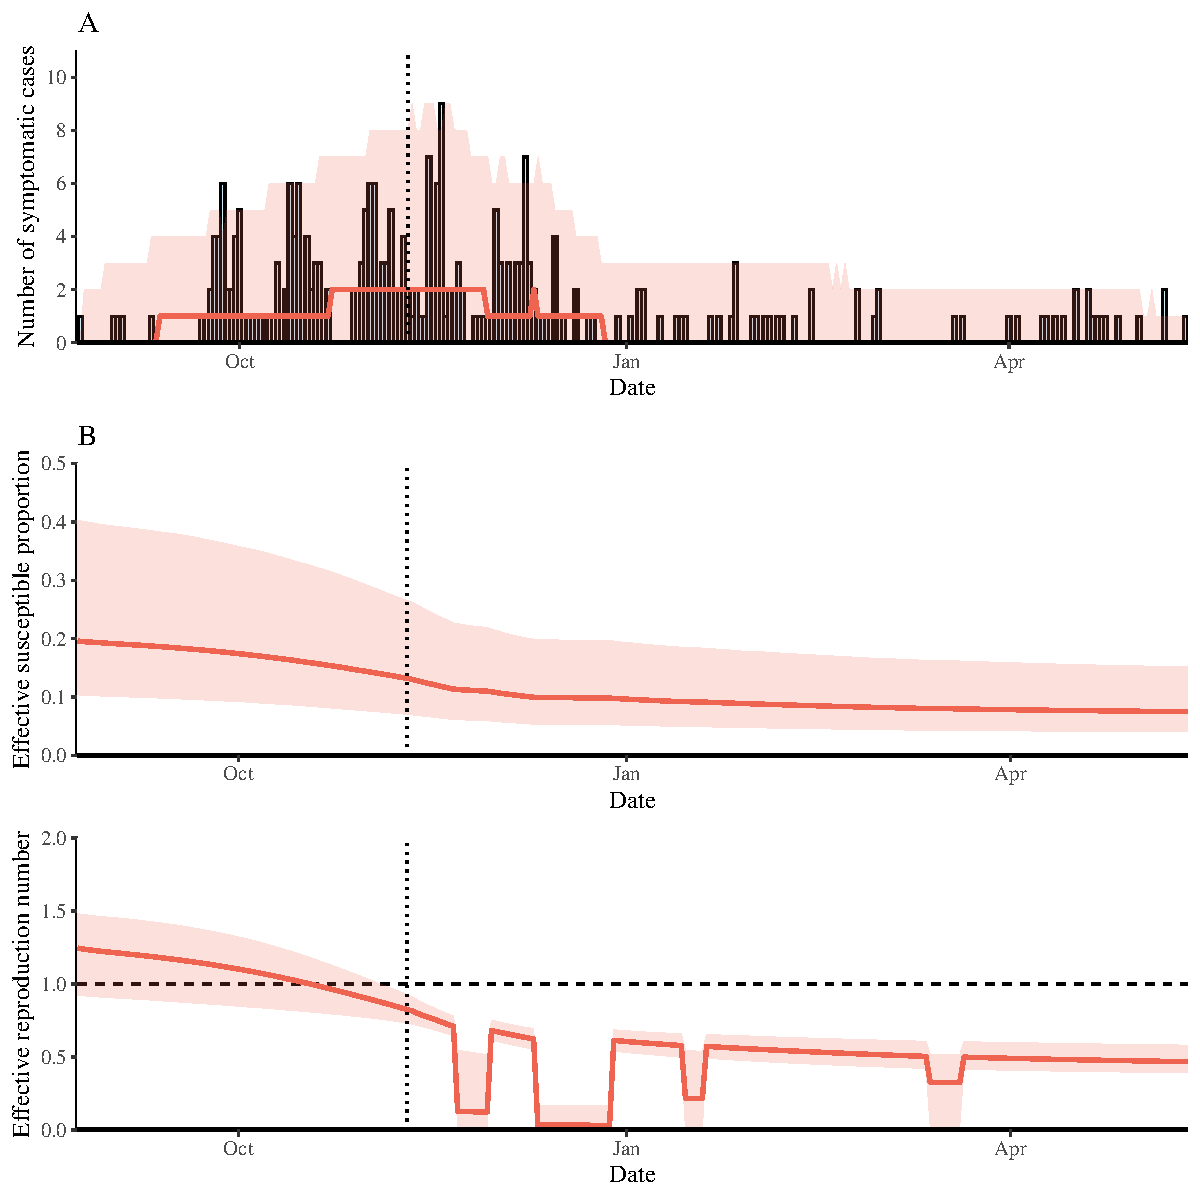
\includegraphics[width=1\textwidth]{../figure_stanfit_seirv_final/figure_stanfit_trajectory.pdf}
\caption{
\textbf{Mechanistic model fits to mumps outbreak at the University of Iowa.}
(A) Comparison of reported number of symptomatic cases on each day (epidemic curve) and posterior medians (red line) and 95\% prediction intervals (red ribbons) of number of symptomatic cases on each day.
(B) Estimated medians (red line) and 95\% credible intervals (red ribbons) of the effective proportion of susceptible students on a given day.
(C) Estimated medians (red line) and 95\% credible intervals (red ribbons) of the effective reproduction number $\mathcal R(t)$ on a given day.
Vertical dotted lines represent the timing of vaccination campaign.
}
\label{fig:fit}
\end{figure}

Our deterministic model provided a reasonable fit to the case data with 95\% prediction intervals covering most of the observations (\fref{fit}A).
Our model fits further suggested that the daily number of symptomatic cases reached its peak near the start of the vaccination campaign, indicating that vaccines may have been introduced after the number of infections had already peaked.
However, our model consistently underestimated the total number of cases among MMR3 recipients (Supplementary Figure S2).
During the outbreak, 221 and 34 cases were reported among second and third dose recipients, respectively---our model predicted 244 (95\% prediction interval: 191--305) and 13 (95\% PI: 5--24) cases, respectively, even though the model was also fitted to the total number of cases.
We address these discrepancies in the discussion.

Despite large uncertainties, we found a slow decreasing pattern in the estimates of the effective proportion of susceptible students $\bar{S}(t)$, which did not necessarily coincide with the timing of vaccination campaign (\fref{fit}B), and found that the model-based estimates of $\mathcal{R}(t)$ started to decrease before the vaccination campaign (\fref{fit}C).
We also estimated a strong reduction in $\mathcal{R}(t)$ during winter break and a moderate reduction during Thanksgiving break, likely driven by closure of classes and students going back home (\fref{fit}C);
we did not find clear impact of holiday effects during spring holidays.

Estimates of $\mathcal{R}_{\mathrm c}(t)$ (Supplementary Figure S3) based on the Wallinga-Teunis approach were qualitatively similar to estimates of $\mathcal{R}(t)$.
Both showed initial reduction in the estimated reproduction number prior to the vaccination campaign and holiday effects around the time of winter break, providing support for the robustness of our model fits.
Estimates of $\mathcal{R}_{\mathrm c}(t)$ suggested a potential increase in transmission following the end of winter break, which may be caused by the increase in contact rates with students coming back on campus.
Estimates of $\mathcal{R}_{\mathrm c}(t)$ also suggested a possibility of multiple introduction events, as indicated by a large jump in $\mathcal{R}_{\mathrm c}(t)$ in the beginning of the outbreak and near the end of March.

% Parameter estimates of our compartmental model fits are presented in Supplementary Figure S4.
We found large uncertainties in many model parameters, especially in the basic reproduction number (Supplementary Figure S4A); our estimates (median: 8.7; 95\% CI: 4.5--15.9) were higher than the assumed prior distribution (median: 4.7; 95\% quantile: 1.6--10.2) but the distributions largely overlap.
\DIFaddbegin \DIFadd{We found 19.6\% (95\% CI: 10.4\%--40.3\%) of the student population to be susceptible against mumps infection at the beginning of an outbreak;
interestingly, this estimate is consistent with \mbox{%DIFAUXCMD
\cite{gokhale2023disentangling} }\hskip0pt%DIFAUXCMD
who estimated 16\% of the US population over 25y to be susceptible as of 2000.
}\DIFaddend The estimates of holiday effects varied considerably (Supplementary Figure S4B--E): Thanksgiving break (82.2\%; 95\% CI: 21.4\%--99.3\%), winter break (94.8\%; 95\% CI: 72.1\%--99.8\%), between-term break (62.3\%; 95\% CI: 5.1\%--98.1\%), and spring break (34.1\%; 95\% CI: 1.5\%--95.2\%). 
\DIFaddbegin \DIFadd{Assuming a single value for holiday effects suggested a much stronger reduction in transmission (Supplementary Figure S5): 95.8\% (95\% CI: 77.6\%--99.9\%)
}\DIFaddend We estimated a low reporting probability (11.2\%; 95\% CI: 4.9\%--31.2\%; Supplementary Figure S4F), but this estimate must be interpreted with care because it can be sensitive to underlying dynamical and epidemiological factors (see Discussion).
The combined VE was 49.2\% (95\% CI: 16.0\%--88.3\%) for a mean delay of 7 days between vaccination and protection (Supplementary Figure S4G). 
Assuming a longer delay between vaccination and protection led to similar parameter estimates overall but with greater uncertainties.
The combined VE was 44.8\% (95\% CI: 8.0\%--86.8\%) and 40.4\% (95\% CI: 3.7\%--86.4\%) when the mean delay was 14 and 21 days, respectively (Supplementary Figure S4).
\DIFaddbegin \DIFadd{Using a stochastic model gave broadly similar uncertainty ranges (Supplementary Figure S6).
}\DIFaddend 

Both exclusion and inclusion analyses provided consistent estimates of impact of interventions (\fref{popimp}\DIFaddbegin \DIFadd{, Supplementary Figure S7}\DIFaddend ); for simplicity, we present the results of the exclusion analysis here.
We found that the 2-week winter break likely had the largest impact on final sizes of the mumps outbreak (across 99.5\% of simulations), estimating that the final size of the outbreak would have increased by 28.6\% (95\% CI: 17.0\%--36.3 \%) in the absence of the winter break.
Thanksgiving break also had considerable impact on the final outbreak size, and in the absence of this break, we estimated outbreak size would have increased by 11.7\% (95\% CI: 2.7\%--16.1\%).
Vaccination likely had smaller impact on the final size than Thanksgiving break, but there was large uncertainty in the proportion of cases prevented by the vaccine: 6.4\% (95\% CI: 0.3\%--20.7\%).
Spring break (1.3\%; 95\% CI: 0.0\%--4.4\%) and between-term breaks (2.9\%; 95\% CI: 0.2\%--5.9\%) likely had little impact on the outbreak size.

\begin{figure}[!th]
\DIFdelbeginFL %DIFDELCMD < 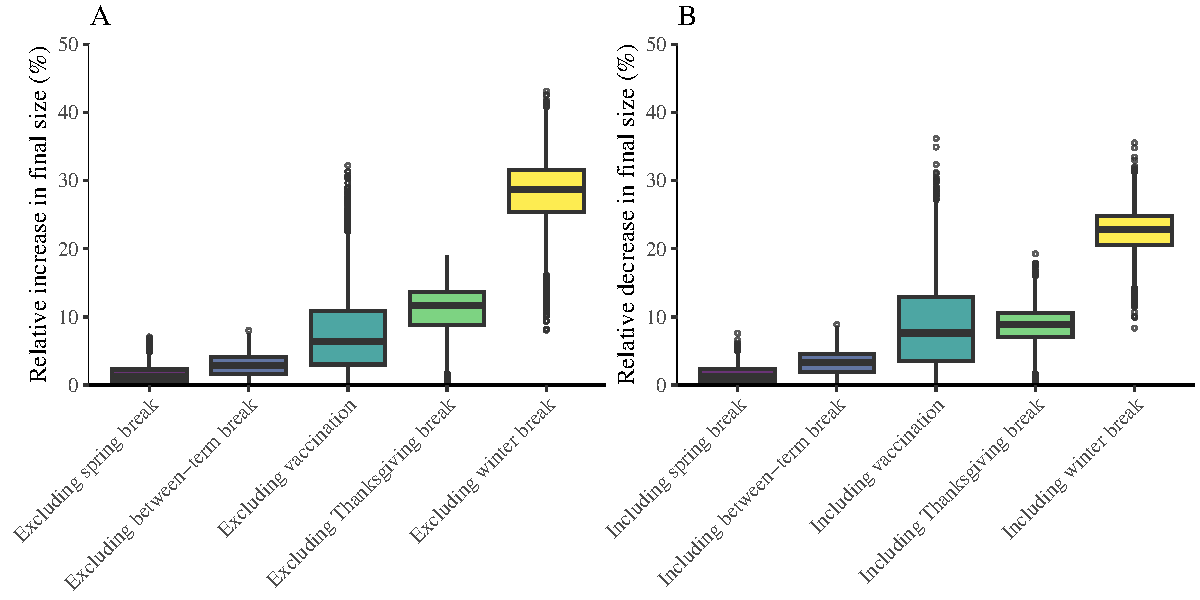
\includegraphics[width=\textwidth]{../figure_stanfit_seirv_final/figure_stanfit_effects.pdf}
%DIFDELCMD < %%%
\DIFdelendFL \DIFaddbeginFL \begin{center}
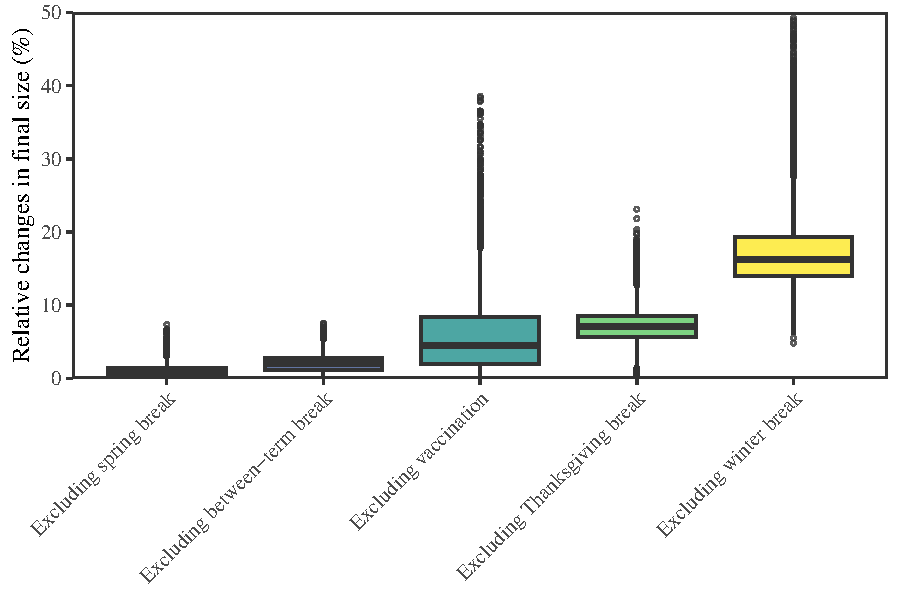
\includegraphics[width=0.7\textwidth]{../figure_stanfit_seirv_final/figure_stanfit_effects_exclusion.pdf}
\DIFaddendFL \caption{
\DIFdelbeginFL \textbf{\DIFdelFL{Population-level impact of vaccination and school holidays in preventing transmission for exclusion (A) and inclusion (B) analysis.}}
%DIFAUXCMD
\DIFdelendFL \DIFaddbeginFL \textbf{\DIFaddFL{Population-level impact of vaccination and school holidays in preventing transmission for exclusion analysis.}}
\DIFaddendFL Box plots of relative \DIFdelbeginFL \DIFdelFL{increase/decrease }\DIFdelendFL \DIFaddbeginFL \DIFaddFL{changes }\DIFaddendFL in final outbreak size in the absence \DIFdelbeginFL \DIFdelFL{/presence }\DIFdelendFL of intervention.
}
\label{fig:popimp}
\DIFaddbeginFL \end{center}
\DIFaddendFL \end{figure}

The impact of different vaccination strategies across a wide range of assumptions about coverage \DIFdelbegin \DIFdel{, timing , VE, and mean delay }\DIFdelend \DIFaddbegin \DIFadd{and timing is presented in \fref{strat};
in Supplementary Figure S8, we present a detailed analysis further stratified by VE and delays }\DIFaddend between vaccination and protection\DIFdelbegin \DIFdel{is presented in \fref{strat}}\DIFdelend .
The timing of vaccination played an important role.
During the mumps outbreak at the University of Iowa, vaccine campaigns were held almost 80 days after the first cases were reported with roughly 23\% coverage, resulting in an estimated 6.4\% (95\% CI: 0.3\%--20.7\%) reduction in the outbreak size (as estimated from the exclusion analysis in \fref{popimp}A).
Had the vaccine been introduced at the start of the outbreak, better outcomes could have been achieved at a 20\% coverage level (which is similar to the coverage level obtained during the real outbreak), ranging from an 11.4\% (95\% CI: 9.3\%--13.1\%) to 42.9\% (95\% CI: 36.7\%--47.5\%) reduction in outbreak size for a vaccine with 20\%--80\% effectiveness against infection with a 7-day delay between vaccination and protection \DIFaddbegin \DIFadd{(Supplementary Figure S8)}\DIFaddend .
Overall, delays between vaccination and protection seemed to have little impact on the outcome of a vaccination strategy \DIFaddbegin \DIFadd{(Supplementary Figure S8)}\DIFaddend .

\begin{figure}[!h]
\DIFdelbeginFL %DIFDELCMD < 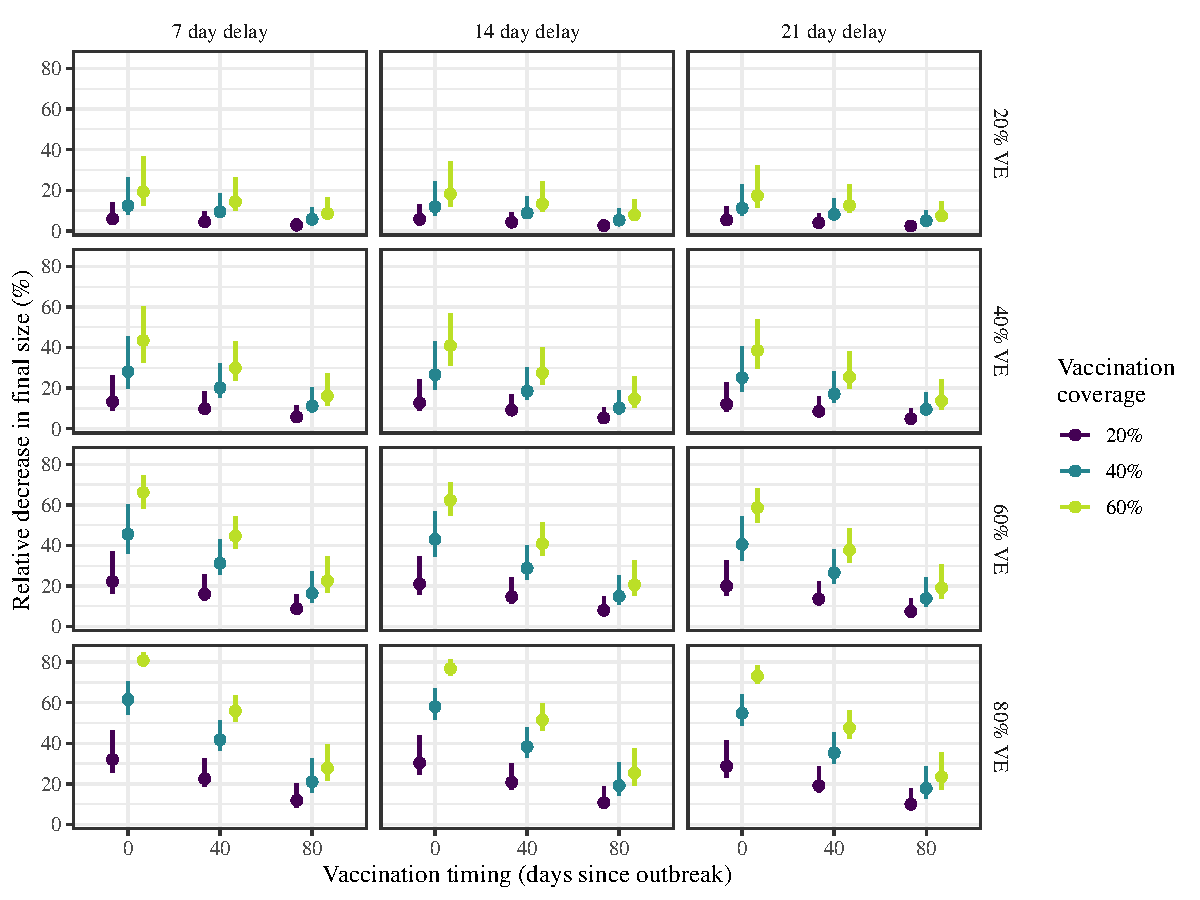
\includegraphics[width=\textwidth]{../figure_stanfit_seirv_final/figure_stanfit_strategy.pdf}
%DIFDELCMD < %%%
\DIFdelendFL \DIFaddbeginFL 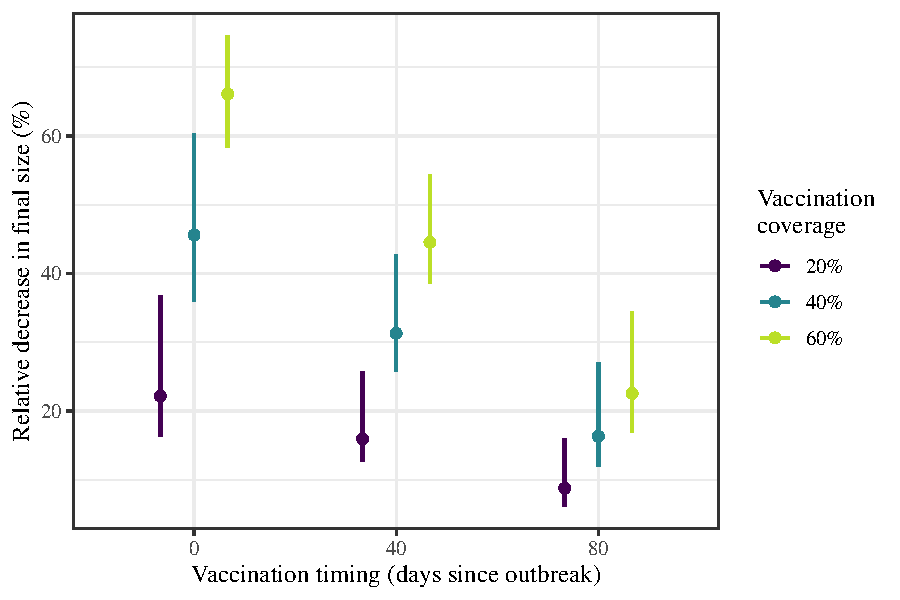
\includegraphics[width=\textwidth]{../figure_stanfit_seirv_final/figure_stanfit_strategy_summ.pdf}
\DIFaddendFL \caption{
\DIFdelbeginFL \textbf{\DIFdelFL{Impact of different vaccination strategies in reducing transmission.}}
%DIFAUXCMD
\DIFdelendFL \DIFaddbeginFL \textbf{\DIFaddFL{Impact of different vaccination strategies in reducing transmission for 60\% VE and 7 day delay between vaccination and protection.}}
\DIFaddendFL We simulate the model under \DIFdelbeginFL \DIFdelFL{108 }\DIFdelendFL \DIFaddbeginFL \DIFaddFL{9 }\DIFaddendFL different vaccination strategies across the posterior distributions.
Then, we evaluate the impact of each vaccination strategy in decreasing the final size of the outbreak, relative to no vaccination scenario.
Points represent median estimates.
Error bars represent 95\% credible intervals.
}
\label{fig:strat}
\end{figure}

\section{Discussion}

We modeled the impact of third dose MMR vaccine in preventing mumps during the 2015--2016 outbreak at the University of Iowa. 
We estimated that the third dose MMR vaccine provided 49.2\% (95\% CI: 16.0\%–88.3\%) protection against mumps cases. 
While vaccination played a role in improving protection of persons at increased risk and preventing transmission during the outbreak, its overall impact on outbreak control was uncertain, especially due to the timing of third-dose introduction. 
We found that winter break likely had the largest impact on overall outbreak dynamics, reducing transmission and highlighting the importance of a physical separation intervention that removes susceptible persons in close contact with infected persons for more than one infectious or incubation period. 
We also found that earlier introduction of vaccination would have further reduced outbreak size, limiting the susceptibility of the student population to infection and leading to a more manageable outbreak throughout the academic year. 

Our estimate of combined VE, 49.2\% (95\% CI: 16.0\%--88.3\%) 7 days after MMR3, is lower but consistent with the previous estimate by \cite{cardemil2017effectiveness} for the same interval, 60\% (95\% CI: 38.4\%--74\%).
\DIFdelbegin \DIFdel{We did not find an increase in VE with time since MMR3 however, the credible/confidence intervals for all estimatesare wide and overlap}\DIFdelend \DIFaddbegin \DIFadd{Assuming longer delays between vaccination and protection still gave similar estimates for VE that are broadly consistent with previous estimates}\DIFaddend .
Large uncertainties suggest that this outbreak alone does not provide sufficient information to fully understand the effectiveness of the third dose vaccine in controlling mumps outbreaks.
Future studies should prioritize collecting additional data about MMR3 introduction in outbreak settings to clarify parameter estimates and reduce uncertainty in the estimation of MMR3 VE.
% Even though the evidence for the waning immunity of the mumps vaccine is growing \citep{rasheed2019}, there is currently limited information on the real-world effectiveness of the third dose MMR vaccine

\DIFaddbegin \DIFadd{Our estimate of $\mathcal R_0$, 8.7 (95\% CI: 4.5--15.9), is higher but consistent with previous estimates.
For example, \mbox{%DIFAUXCMD
\cite{edmunds2000pre} }\hskip0pt%DIFAUXCMD
estimated pre-vaccination $\mathcal R_0$ between 3.3 and 10.3 for different mixing assumptions from serological data.
Similarly, \mbox{%DIFAUXCMD
\cite{farrington2001estimation} }\hskip0pt%DIFAUXCMD
also estimated $\mathcal R_0$ between 3.3 and 25.5 for different assumptions about contact patterns from serological data.
More recent estimates also range between 3--14 \mbox{%DIFAUXCMD
\citep{majumder2017vaccine,lewnard2018vaccine}}\hskip0pt%DIFAUXCMD
.
The advantage of our Bayesian approach is that it allows us to evaluate the impact of vaccination across a wide range of plausible values for $\mathcal R_0$.
Moreover, the transmission on campus is better characterized by $\mathcal R (t)$, which we estimated to fluctuate around 1--1.5 in the beginning of an outbreak (\fref{fit}C, Supplementary Figure S3);
this is slightly lower but consistent with an estimate by \mbox{%DIFAUXCMD
\cite{shah2022containing}}\hskip0pt%DIFAUXCMD
, who analyzed mumps outbreak at Harvard University in 2016: 1.63.
}

\DIFaddend There are several limitations to our analysis. 
First, we assumed that the underlying transmission process is deterministic. 
In reality, random fluctuations in the number of infections (also known as the demographic stochasticity) can play an important role on outbreak persistence.
Indeed, large jumps in our estimates of the $\mathcal{R}_{\mathrm c}(t)$ indicate the possibility of multiple introductions as well as fade out events;
neglecting such stochasticity may have affected our estimates of uncertainties in VE \citep{king2015avoidable}.
We also assumed a homogeneous population with all undergraduate students at equal risk of infection, which is unlikely to represent the real risk of mumps. 
Congregate settings such as universities are at higher risks for mumps outbreaks, but even within a university, certain groups of students with prolonged, intense close contact are at highest risk of disease (e.g., fraternities/sororities or athletic teams). 
\DIFaddbegin \DIFadd{In addition, many undergraduate students move to off campus housing after their first year, which can increase the amount of contacts with community members and add heterogeneity to mixing patterns---for example, in 2017, it was reported that 95\% and 15\% of freshmen and sophomores live on campus \mbox{%DIFAUXCMD
\citep{news}}\hskip0pt%DIFAUXCMD
.
}\DIFaddend Neglecting structured transmission and differential force of infection may also have biased our estimates of VE.

Our parameter estimates are necessarily crude as we do not explicitly model subclinical cases or community transmission.
Additionally, our compartmental model assumed that all dynamics are driven by susceptible depletion alone.
However, the initial reduction in $\mathcal R(t)$ could be driven by either susceptible depletion, changes in behavior, or stochastic variation in population behavior and we could not distinguish among them without additional epidemiologic or serological information.
With other factors affecting the transmission rate, susceptible depletion would not account for all variation in $\mathcal R(t)$, and the reporting probability estimates would increase.
Specific factors that could influence transmission that we did not account for include impact of control measures taken (e.g., implementation of standardized protocols for case detection with rapid testing and isolation of cases, heightened student awareness), adherence to recommendations for isolation, or differential health-care seeking behavior (i.e., students who received MMR3 might be more likely to present for medical care and report symptoms, which would have led to a downward bias in our VE estimates).

Finally, while our model provides a reasonable fit to the overall outbreak trajectory (\fref{fit}), it underestimates the total number of reported cases among MMR3 recipients (Supplementary Figure S1).
There are many potential sources of this bias: for example, increased contact rates (e.g., due to changes in the risk perception following vaccination) and assortative mixing among MMR3 recipients that would further increase the number of mumps cases among them.
Additionally, regarding the assumption of random administration of vaccination, if groups at higher risk of infection (e.g., fraternities/athletic teams) received vaccine earlier, then these individuals likely experienced a higher force of infection than 2-dose recipients, which would have lowered the VE estimate. 
However, testing such hypotheses would require additional data.
Despite these limitations, our qualitative conclusions are likely to be robust: delayed introduction of vaccination can limit its population-level impact and bias the inference of its effectiveness.

Overall, we found that MMR3 provided some level of individual protection and can potentially help limit mumps transmission if vaccination is introduced early during an outbreak.  
However, our analysis also shows that physical distancing (i.e., school breaks) can play an important role in interrupting mumps transmission. 
While school breaks cannot be implemented randomly, early detection of cases and adherence to the isolation recommendations of patients diagnosed with mumps are important measures to assist with control of mumps in a highly 2-dose vaccinated populations \DIFaddbegin \DIFadd{\mbox{%DIFAUXCMD
\citep{shah2022containing}}\hskip0pt%DIFAUXCMD
}\DIFaddend .

\section*{Data availability}

All code are stored in a publicly available GitHub repository (\url{https://github.com/parksw3/mumps}). All data used in the analyses are presented in this paper.

\section*{Conflict of interest}

The authors declare no competing interest.

\pagebreak

\section*{Supplementary Materials}

\subsection*{\DIFdelbegin \DIFdel{Mathematical details}\DIFdelend \DIFaddbegin \DIFadd{Deterministic model}\DIFaddend }

During holidays (represented by $h_i(t) = 1$ if holiday $i$ is occurring at time $t$), we assume that the transmission rate is proportionally reduced by $r_i$. 
Newly infected individuals remain exposed for an average of $1/\sigma$ days and become infectious for an average of $1/\gamma$ days.
Then, the corresponding continuous-time model is given by:
  \begin{align}
  \frac{dS}{dt} &= - \frac{\beta (1 - \sum_i r_i h_i(t)) S (I_s + I_v + I_p)}{N} - \nu(t) S\\
  \frac{dE_s}{dt} &= \frac{\beta (1 - \sum_i r_i h_i(t)) S (I_s + I_v + I_p)}{N} - \sigma E_s\\
  \frac{dI_s}{dt} &= \sigma E_s - \gamma I_s\\
  \frac{dV}{dt} &= \nu(t) S - \frac{\beta (1 - \sum_i r_i h_i(t)) V (I_s + I_v + I_p)}{N} - \delta V\\
  \frac{dE_v}{dt} &= \frac{\beta (1 - \sum_i r_i h_i(t)) V (I_s + I_v + I_p)}{N} - \sigma E_v\\
  \frac{dI_v}{dt} &= \sigma E_v - \gamma I_v\\
  \frac{dP}{dt} &= \delta V - \frac{(1-\mathrm{VE}_{\textrm{\tiny{inf}}})\beta (1 - \sum_i r_i h_i(t)) P (I_s + I_v + I_p)}{N}\\
  \frac{dE_p}{dt} &= \frac{\beta (1 - \sum_i r_i h_i(t)) P (I_s + I_v + I_p)}{N} - \sigma E_p\\
  \frac{dI_p}{dt} &= \sigma E_p - \gamma I_p\\
  \frac{dR}{dt} &= \gamma I_s + \gamma I_v + \gamma I_p\\
  \end{align}
We discretize this model using \DIFdelbegin \DIFdel{Euler multinomial }\DIFdelend \DIFaddbegin \DIFadd{Euler-multinomial }\DIFaddend scheme \citep{he2010plug}:
\begin{align}
\textrm{FOI}(t) &= \frac{\beta (1 - \sum_i r_i h_i(t)) I(t-\Delta t)}{N}\\
\Delta S(t) &= \left[1- \exp(-(\textrm{FOI}(t) + \nu(t)) \Delta t )\right] S(t-\Delta t)\\
N_{SE_s}(t) &= \frac{\textrm{FOI}(t)\Delta S(t)}{\textrm{FOI}(t) + \nu(t)} \\
N_{SV}(t) &= \frac{\nu(t)\Delta S(t)}{\textrm{FOI}(t) + \nu(t)} \\
N_{E_sI_s}(t) &= \left[1- \exp(-\sigma \Delta t )\right] E_s(t-\Delta t)\\
N_{I_sR}(t) &= \left[1- \exp(-\gamma \Delta t )\right] I_s(t-\Delta t)\\
\Delta V(t) &= \left[1- \exp(-(\textrm{FOI}(t) + \delta(t)) \Delta t )\right] S(t-\Delta t)\\
N_{VE_v}(t) &= \frac{\textrm{FOI}(t)\Delta V(t)}{\textrm{FOI}(t) + \delta(t)} \\
N_{VP}(t) &= \frac{\delta(t)\Delta V(t)}{\textrm{FOI}(t) + \delta(t)} \\
N_{E_vI_v}(t) &= \left[1- \exp(-\sigma \Delta t )\right] E_v(t-\Delta t)\\
N_{I_vR}(t) &= \left[1- \exp(-\gamma \Delta t )\right] I_v(t-\Delta t)\\
N_{PE_p}(t) &= \left[1-\exp(-(1-\mathrm{VE}_{\textrm{\tiny{inf}}})\textrm{FOI}(t) \Delta t)\right] P(t-\Delta t)  \\
N_{E_pI_p}(t) &= \left[1- \exp(-\sigma \Delta t )\right] E_p(t-\Delta t)\\
N_{I_pR}(t) &= \left[1- \exp(-\gamma \Delta t )\right] I_p(t-\Delta t)\\
S(t) &= S(t-\Delta t) - N_{SE_s}(t) - N_{SV}(t)\\
E_s(t) &= E(t-\Delta t) + N_{SE_s}(t) - N_{E_sI_s}(t)\\
I_s(t) &= I(t-\Delta t) + N_{E_sI_s}(t) - N_{I_sR}(t)\\
V(t) &= V(t-\Delta t) + N_{SV}(t) - N_{SE_v}(t) - N_{VP}(t)\\
E_v(t) &= E(t-\Delta t) + N_{SE_v}(t) - N_{E_vI_v}(t)\\
I_v(t) &= I(t-\Delta t) + N_{E_vI_v}(t) - N_{I_vR}(t)\\
P(t) &= P(t-\Delta t) + N_{VP}(t) - N_{PE_p}(t)\\
E_v(t) &= E(t-\Delta t) + N_{PE_p}(t) - N_{E_pI_p}(t)\\
I_v(t) &= I(t-\Delta t) + N_{E_pI_p}(t) - N_{I_pR}(t)\\
R(t) &= R(t-\Delta t) + N_{I_sR}(t) + N_{I_vR}(t) + N_{I_pR}(t)
\end{align}
where $\textrm{FOI}$ represent the force of infection and $N_{ij}$ represent the number of individuals moving from compartment $i$ to $j$ on a given day. We simulate this model using a time step $\Delta t$ of 1 day.

\DIFaddbegin \subsection*{\DIFadd{Stochastic model}}

\DIFadd{We also implemented a discrete-time stochastic model using the Euler-multinomial scheme through the R package pomp \mbox{%DIFAUXCMD
\citep{king2015statistical}}\hskip0pt%DIFAUXCMD
:
}\begin{align}
\DIFadd{\textrm{FOI}(t) }&\DIFadd{= \frac{\beta (1 - \sum_i r_i h_i(t)) I(t-\Delta t)}{N}}\\
\DIFadd{\Delta S(t) }&\DIFadd{= \mathrm{Binomial}\left(S(t-\Delta t),1- \exp(-(\textrm{FOI}(t) + \nu(t)) \Delta t )\right)}\\
\DIFadd{N_{SE_s}(t) }&\DIFadd{= \mathrm{Binomial}\left(\Delta S(t), \frac{\textrm{FOI}(t)}{\textrm{FOI}(t) + \nu(t)} \right)}\\
\DIFadd{N_{SV}(t) }&\DIFadd{= \Delta S(t) - N_{SE_s}(t)}\\
\DIFadd{N_{E_sI_s}(t) }&\DIFadd{= \mathrm{Binomial}\left(E_s(t-\Delta t), 1- \exp(-\sigma \Delta t )\right)}\\
\DIFadd{N_{I_sR}(t) }&\DIFadd{= \mathrm{Binomial}(I_s(t-\Delta t), 1- \exp(-\gamma \Delta t))}\\
\DIFadd{\Delta V(t) }&\DIFadd{= \mathrm{Binomial}\left( S(t-\Delta t), 1- \exp(-(\textrm{FOI}(t) + \delta(t)) \Delta t )\right)}\\
\DIFadd{N_{VE_v}(t) }&\DIFadd{= \mathrm{Binomail}\left(\Delta V(t), \frac{\textrm{FOI}(t)}{\textrm{FOI}(t) + \delta(t)}  \right) }\\
\DIFadd{N_{VP}(t) }&\DIFadd{= \Delta V(t) -N_{VE_v}(t)  }\\
\DIFadd{N_{E_vI_v}(t) }&\DIFadd{= \mathrm{Binomial}(E_v(t-\Delta t), 1- \exp(-\sigma \Delta t ))}\\
\DIFadd{N_{I_vR}(t) }&\DIFadd{= \mathrm{Binomial}(I_v(t-\Delta t), 1- \exp(-\gamma \Delta t ))}\\
\DIFadd{N_{PE_p}(t) }&\DIFadd{= \mathrm{Binomial}(P(t-\Delta t), 1-\exp(-(1-\mathrm{VE}_{\textrm{\tiny{inf}}})\textrm{FOI}(t) \Delta t))}\\
\DIFadd{N_{E_pI_p}(t) }&\DIFadd{= \mathrm{Binomial}(E_p(t-\Delta t), 1- \exp(-\sigma \Delta t))}\\
\DIFadd{N_{I_pR}(t) }&\DIFadd{= \mathrm{Binomial}(I_p(t-\Delta t), 1- \exp(-\gamma \Delta t))}\\
\DIFadd{S(t) }&\DIFadd{= S(t-\Delta t) - N_{SE_s}(t) - N_{SV}(t)}\\
\DIFadd{E_s(t) }&\DIFadd{= E(t-\Delta t) + N_{SE_s}(t) - N_{E_sI_s}(t)}\\
\DIFadd{I_s(t) }&\DIFadd{= I(t-\Delta t) + N_{E_sI_s}(t) - N_{I_sR}(t)}\\
\DIFadd{V(t) }&\DIFadd{= V(t-\Delta t) + N_{SV}(t) - N_{SE_v}(t) - N_{VP}(t)}\\
\DIFadd{E_v(t) }&\DIFadd{= E(t-\Delta t) + N_{SE_v}(t) - N_{E_vI_v}(t)}\\
\DIFadd{I_v(t) }&\DIFadd{= I(t-\Delta t) + N_{E_vI_v}(t) - N_{I_vR}(t)}\\
\DIFadd{P(t) }&\DIFadd{= P(t-\Delta t) + N_{VP}(t) - N_{PE_p}(t)}\\
\DIFadd{E_v(t) }&\DIFadd{= E(t-\Delta t) + N_{PE_p}(t) - N_{E_pI_p}(t)}\\
\DIFadd{I_v(t) }&\DIFadd{= I(t-\Delta t) + N_{E_pI_p}(t) - N_{I_pR}(t)}\\
\DIFadd{R(t) }&\DIFadd{= R(t-\Delta t) + N_{I_sR}(t) + N_{I_vR}(t) + N_{I_pR}(t)
}\end{align}
\DIFadd{The measurement model remains identical to the deterministic model: 
}\begin{equation}
\DIFadd{\textrm{reported cases on day } t \sim \mathrm{NegBin}(C_s(t) + C_v(t) + C_p(t), \theta),
}\end{equation}
\DIFadd{where 
}\begin{align}
\DIFadd{C_s(t) }&\DIFadd{= \rho (1-\exp(- \sigma)) E_s(t-1)}\\
\DIFadd{C_v(t) }&\DIFadd{= \rho (1-\exp(- \sigma)) E_v(t-1)}\\
\DIFadd{C_p(t) }&\DIFadd{= (1- \mathrm{VE}_{\textrm{\tiny{symp}}}) \rho (1-\exp(- \sigma)) E_p(t-1).
}\end{align}
\DIFadd{For simplicity, we did not fit the stochastic model to the total number of cases stratified by vaccination status and focused on the overall epidemic trajectory.
}

\DIFadd{By taking the posterior distribution we previously obtained from the deterministic model, we calculated likelihood for each sample using particle filtering with 2000 particles \mbox{%DIFAUXCMD
\citep{king2015statistical}}\hskip0pt%DIFAUXCMD
.
This step allowed us to evaluate the likelihood across realistic ranges of parameters that are consistent with data.
Then, we constructed a profile log-likelihood curve following the approach outlined in \mbox{%DIFAUXCMD
\citep{park2021epidemiological}}\hskip0pt%DIFAUXCMD
.
First, for each parameter, we divided the range into 200 equispaced bins and took maximum log-likelihood in each bin.
We then fitted a locally estimated scatterplot smoothing (LOESS) regression to maximum log-likelihoods across 200 bins to obtain a smooth profile log-likelihood curve.
We then calculated the CIs for each parameter from the estimated profile log-likelihood curves from the LOESS regression.
}

\DIFaddend \subsection*{Case reproduction number}

Estimating $\mathcal{R}_{\mathrm c}(t)$ requires the generation-interval distribution, which describes time from infection to transmission \citep{gostic2020}. 
Instead, we approximate this distribution with a known serial interval distribution, which describes time between symptom onsets of the infector and infectee.
Following \cite{simpson1952infectiousness}, we used delays between the first days of parotid swelling as a proxy for serial intervals, which have a mean 18.6 days and a standard deviation of 4.3 days
and used a gamma distribution to model the serial-interval distribution.
We used the \textit{EpiEstim} package in \texttt{R} to estimate $\mathcal{R}_{\mathrm c}(t)$ while varying the sliding time window between 7--21 days \citep{cori2013new}.

\pagebreak

\subsection*{Supplementary figures}
\setcounter{figure}{0}
\renewcommand{\thefigure}{S\arabic{figure}}


\begin{figure}[!th]
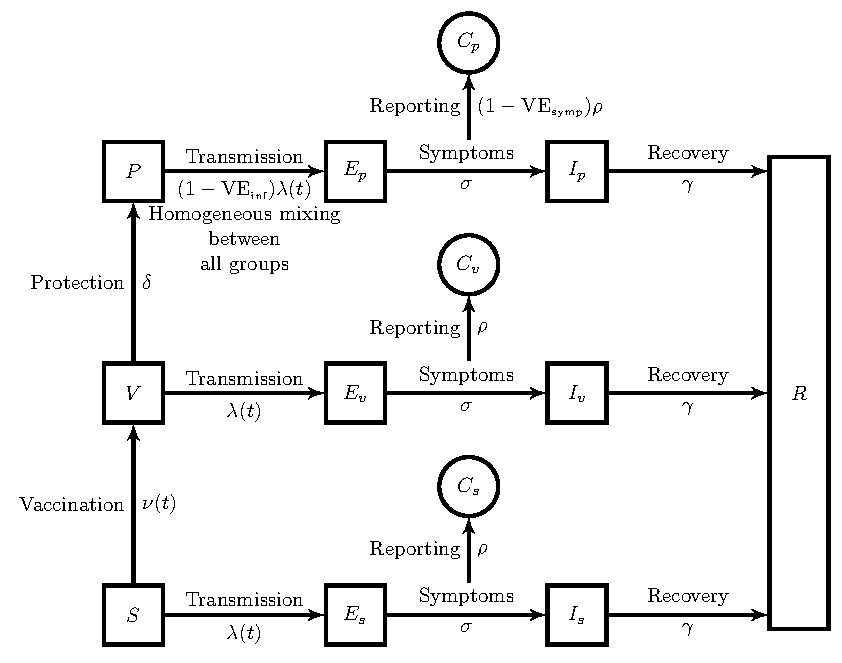
\includegraphics[width=\textwidth]{../figure/diagram.pdf}
\caption{
\textbf{Schematic diagram of the transmission model.}
}
\label{fig:model}
\end{figure}

\pagebreak

\begin{figure}[!h]
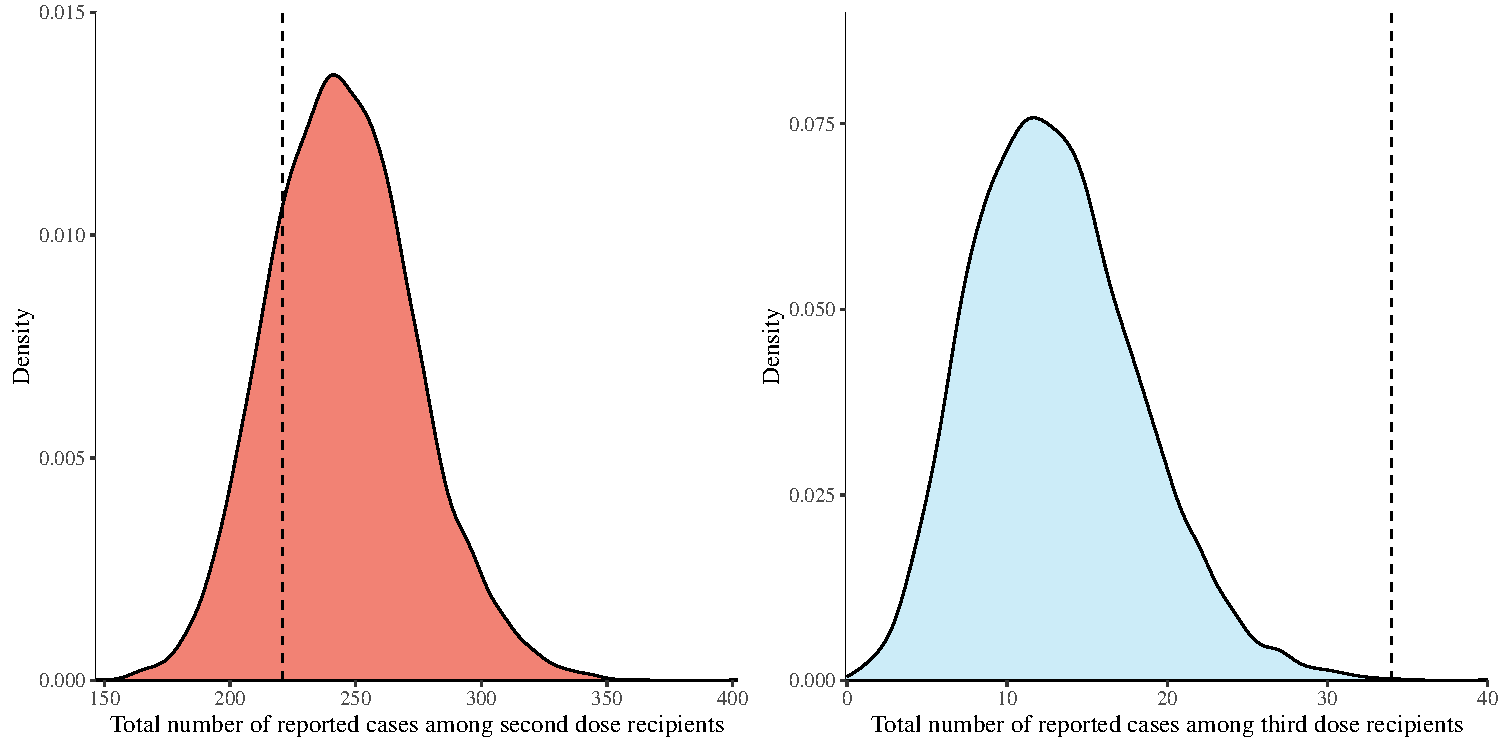
\includegraphics[width=\textwidth]{../figure_stanfit_seirv_final/figure_stanfit_total.pdf}
\caption{
\textbf{Predicted number of reported cases among second (MMR2) and third (MMR3) dose recipients.}
Solid lines represent the posterior distribution for the predicted number of reported cases, which also accounts for the negative binomial error.
Dashed lines represent the actual number of reported cases.
Note that the axses of the posterior density differ between two panels.
}
\end{figure}

\pagebreak

\begin{figure}[!h]
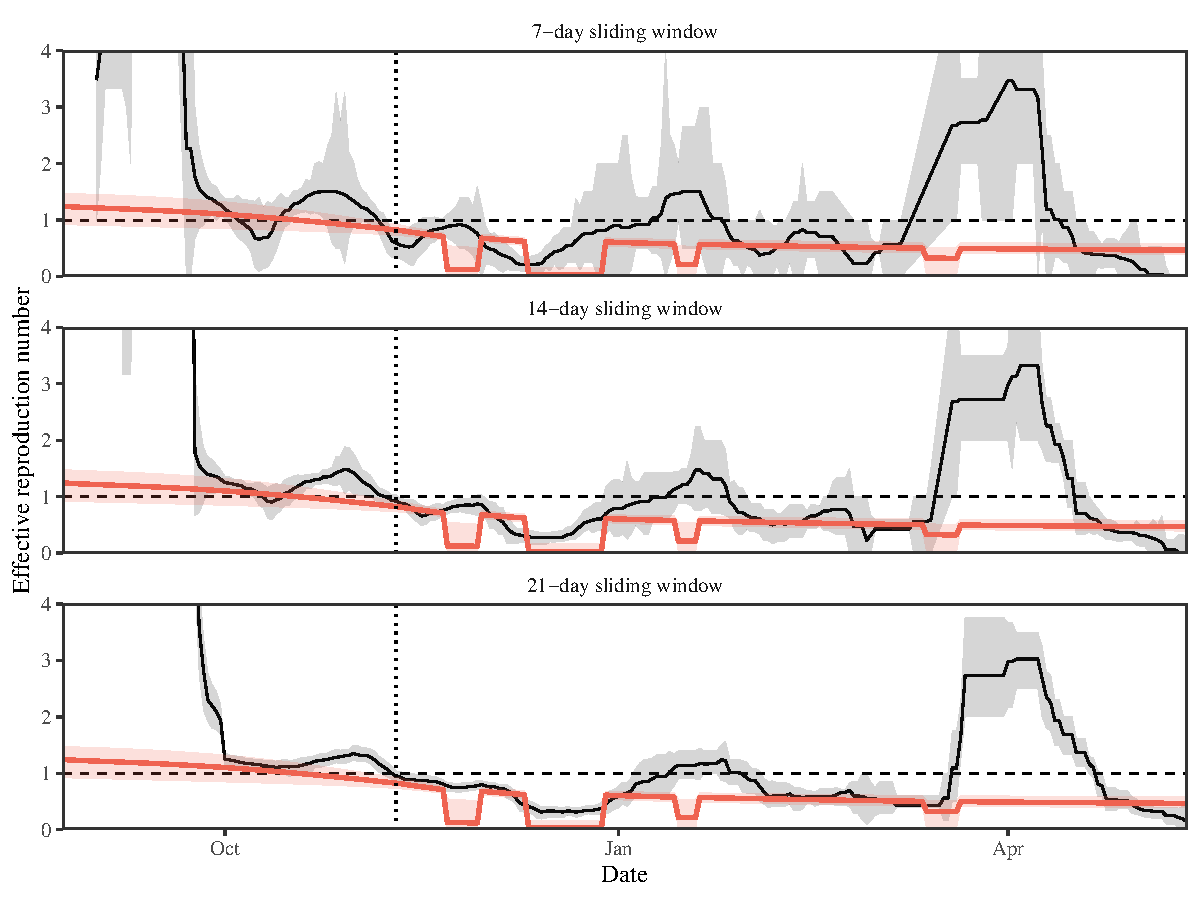
\includegraphics[width=\textwidth]{../figure_stanfit_seirv_final/figure_stanfit_Rt_comp.pdf}
\caption{
\textbf{Comparisons of estimates of case reproduction number $\mathcal R_c(t)$ and model-based estimates of effective reproduction number $\mathcal R(t)$.}
Black lines represent median estimates of case reproduction number $\mathcal R_c(t)$ calculated using the Wallinga-Teunis method.
Red lines represent median estimates of effective reproduction numbers $\mathcal R(t)$ using the compartmental model.
Grey ribbons represent the corresponding 95\% credible intervals.
Horizontal dashed lines represent the $\mathcal R=1$ threshold.
Vertical dotted lines represent the timing of the vaccination campaign.
}
\end{figure}

\pagebreak 

\begin{figure}[!h]
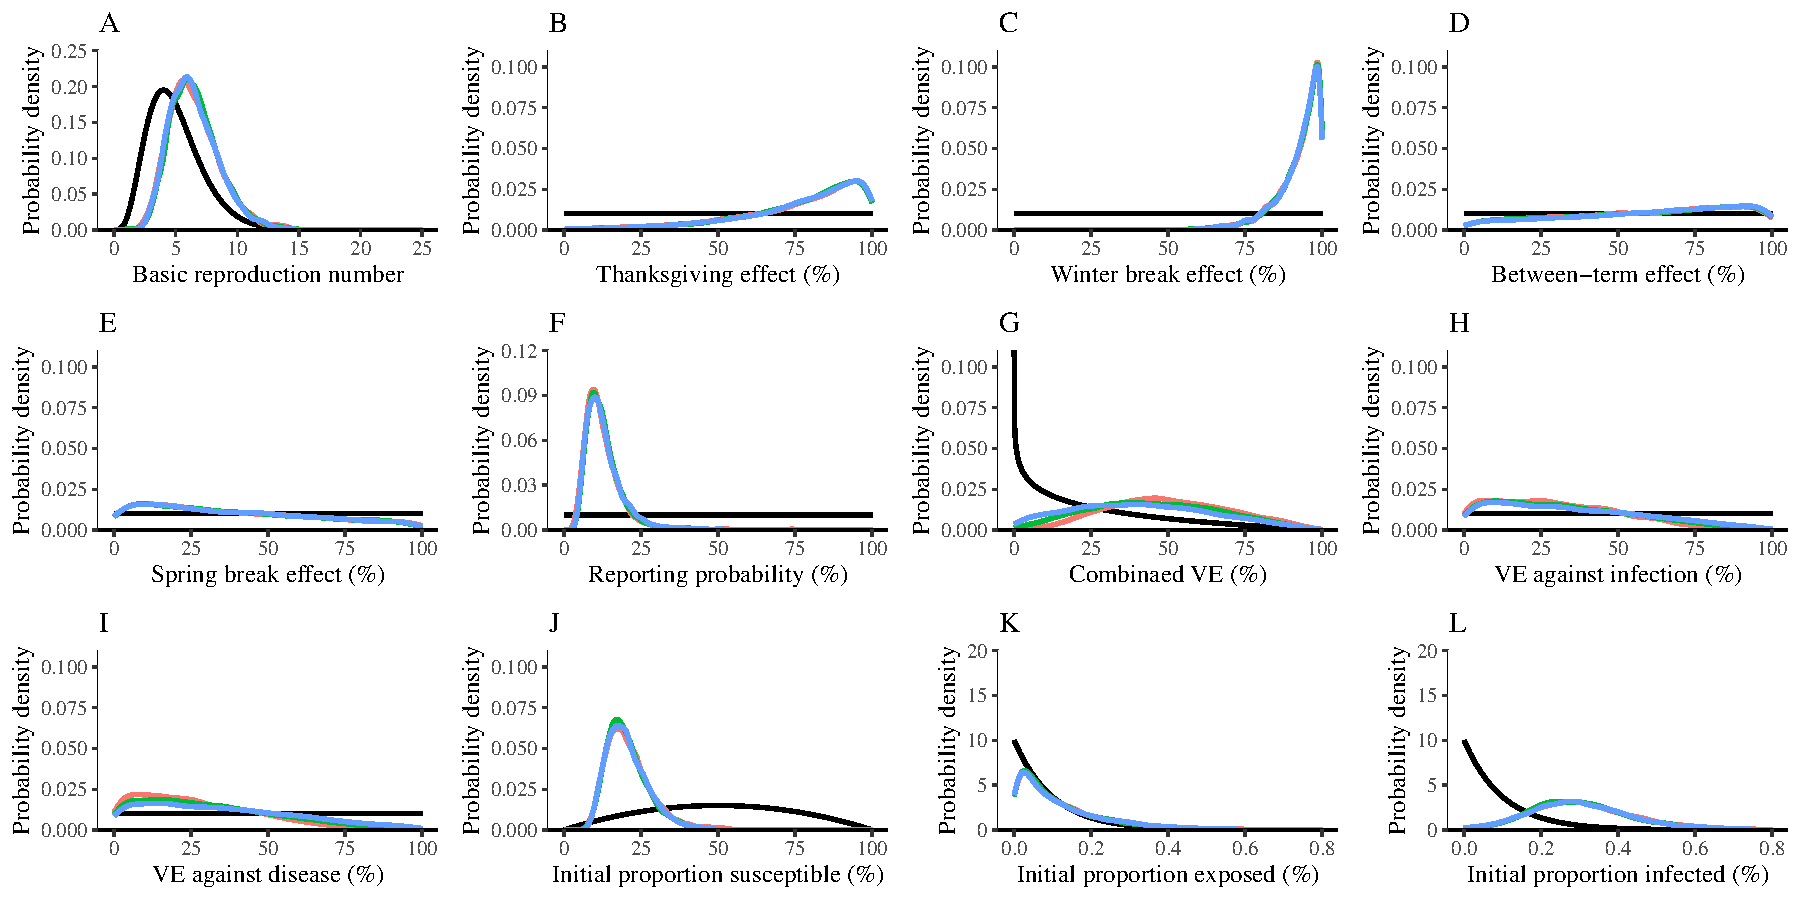
\includegraphics[width=\textwidth]{../figure_stanfit_seirv_final/figure_stanfit_param_all.pdf}
\caption{
\textbf{Parameter estimates for the mumps outbreak at the University of Iowa.}
Black lines represent prior distributions.
Colored lines represent the mean delay between vaccination and protection: 7 days (red), 14 days (green), 21 days (blue).
VE represents vaccine effectiveness.
}
\label{fig:param}
\DIFaddbeginFL \end{figure}

\pagebreak

\begin{figure}[!th]
\begin{center}
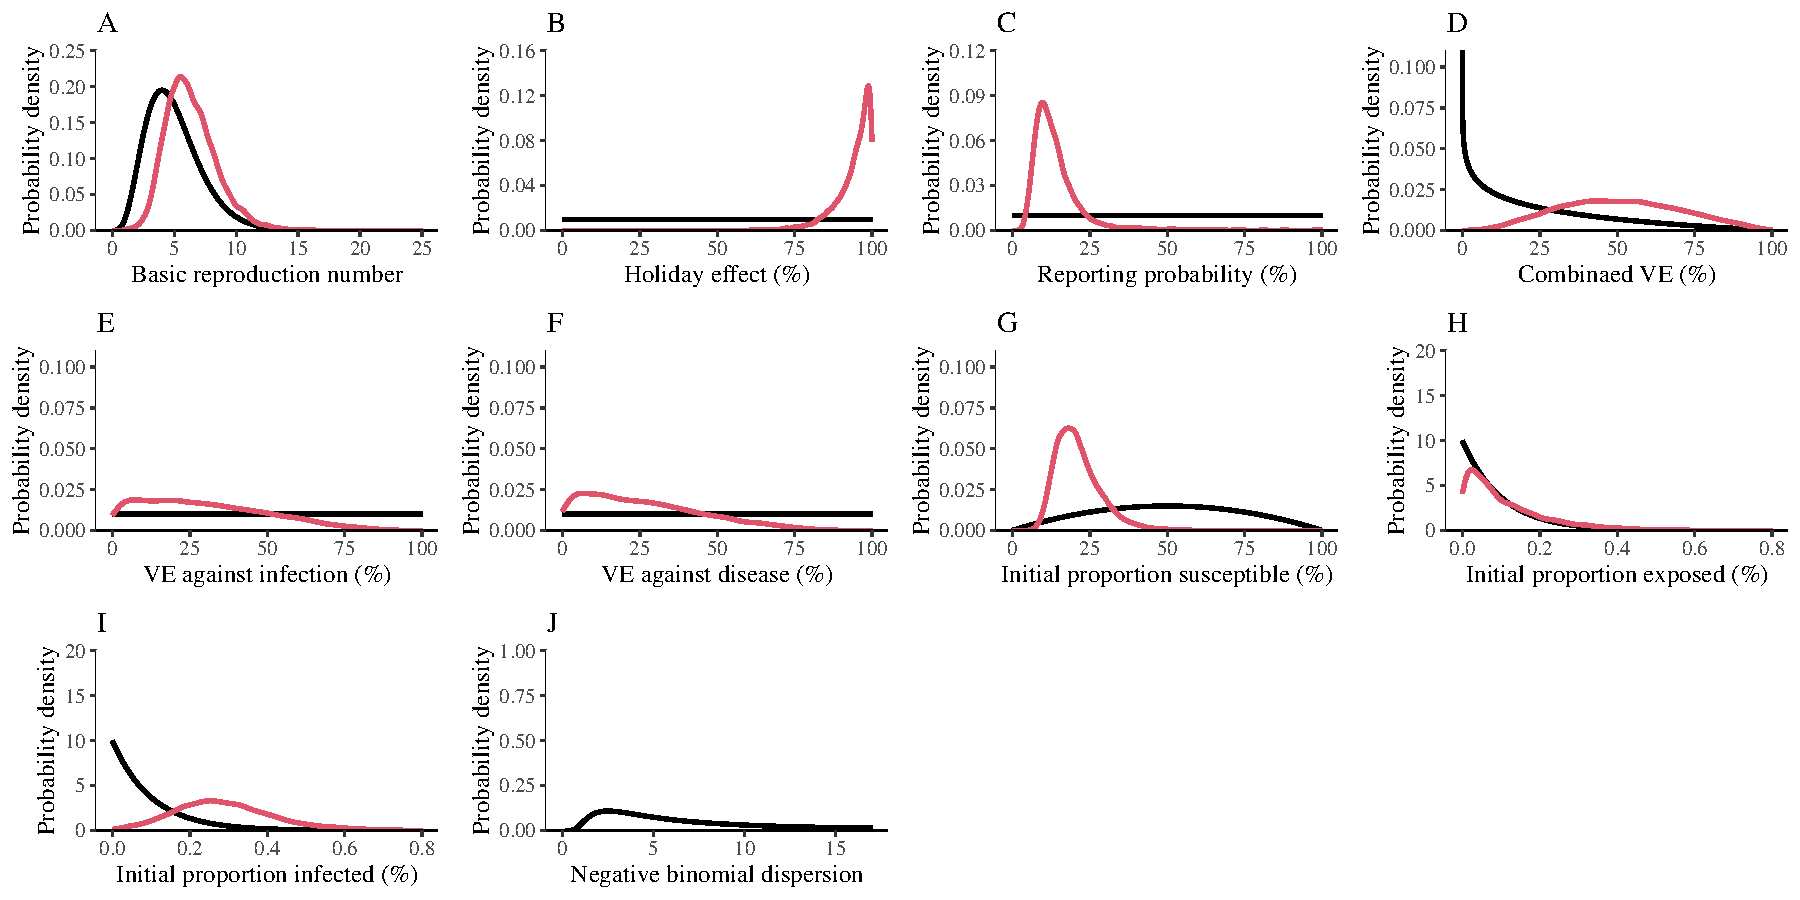
\includegraphics[width=\textwidth]{../figure_stanfit_seirv_final/figure_stanfit_param_avg.pdf}
\caption{
\textbf{\DIFaddFL{Parameter estimates for the mumps outbreak at the University of Iowa assuming a single value for all holidays.}}
\DIFaddFL{Black lines represent prior distributions.
Red lines represent the posterior distribution.
VE represents vaccine effectiveness.
}}
\end{center}
\end{figure}

\pagebreak

\begin{figure}[!h]
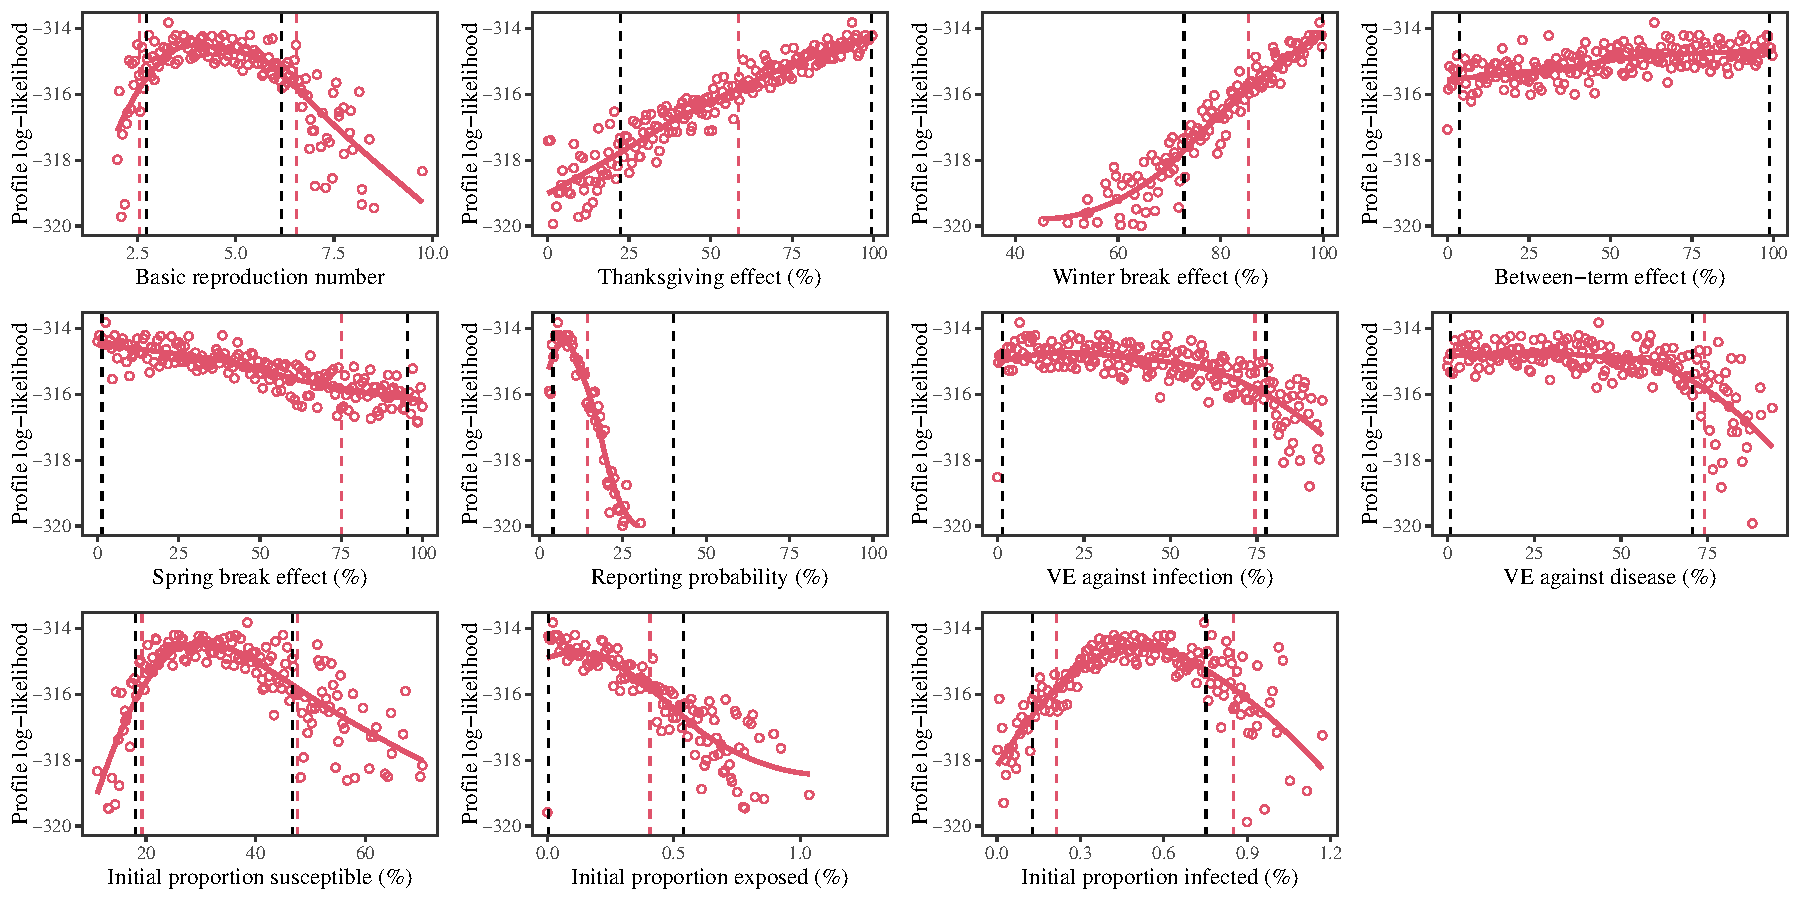
\includegraphics[width=\textwidth]{../pomp/figure_pomp_loglik.pdf}
\caption{
\textbf{\DIFaddFL{Estimated confidence intervals using a stochastic model.}}
\DIFaddFL{Points represent estimates that were used to construct the profile log-likelihood curves, as explained in Supplementary Material.
Solid curves represent the LOESS fit.
Red dashed vertical lines represent the 95\% confidence intervals estimated from the stochastic model.
Black dashed vertical lines represent the 95\% credible intervals estimated from the deterministic model.
}}
\end{figure}

\pagebreak

\begin{figure}[!th]
\begin{center}
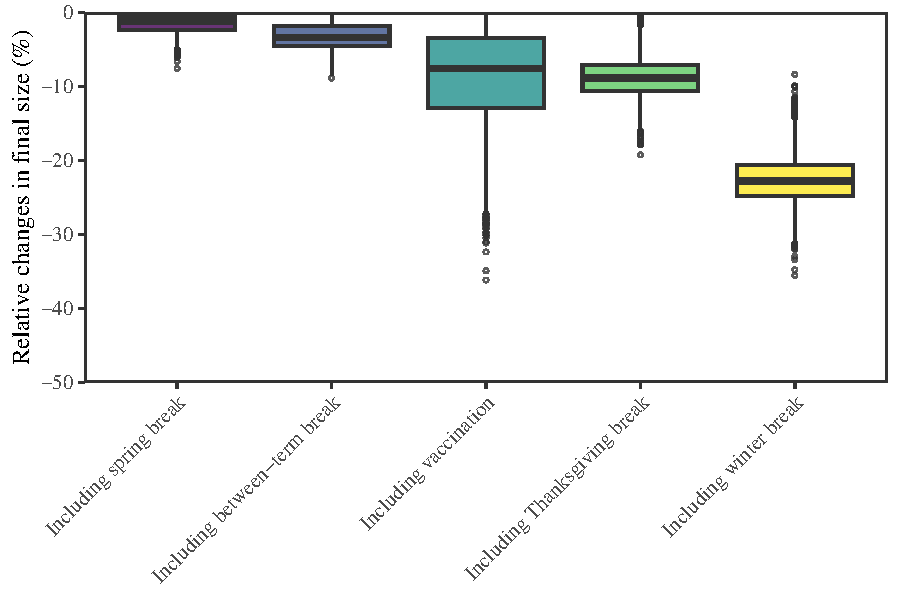
\includegraphics[width=0.7\textwidth]{../figure_stanfit_seirv_final/figure_stanfit_effects_inclusion.pdf}
\caption{
\textbf{\DIFaddFL{Population-level impact of vaccination and school holidays in preventing transmission for inclusion analysis.}}
\DIFaddFL{Box plots of relative changes in final outbreak size in the presence of intervention.
}}
\end{center}
\end{figure}

\pagebreak

\begin{figure}[!h]
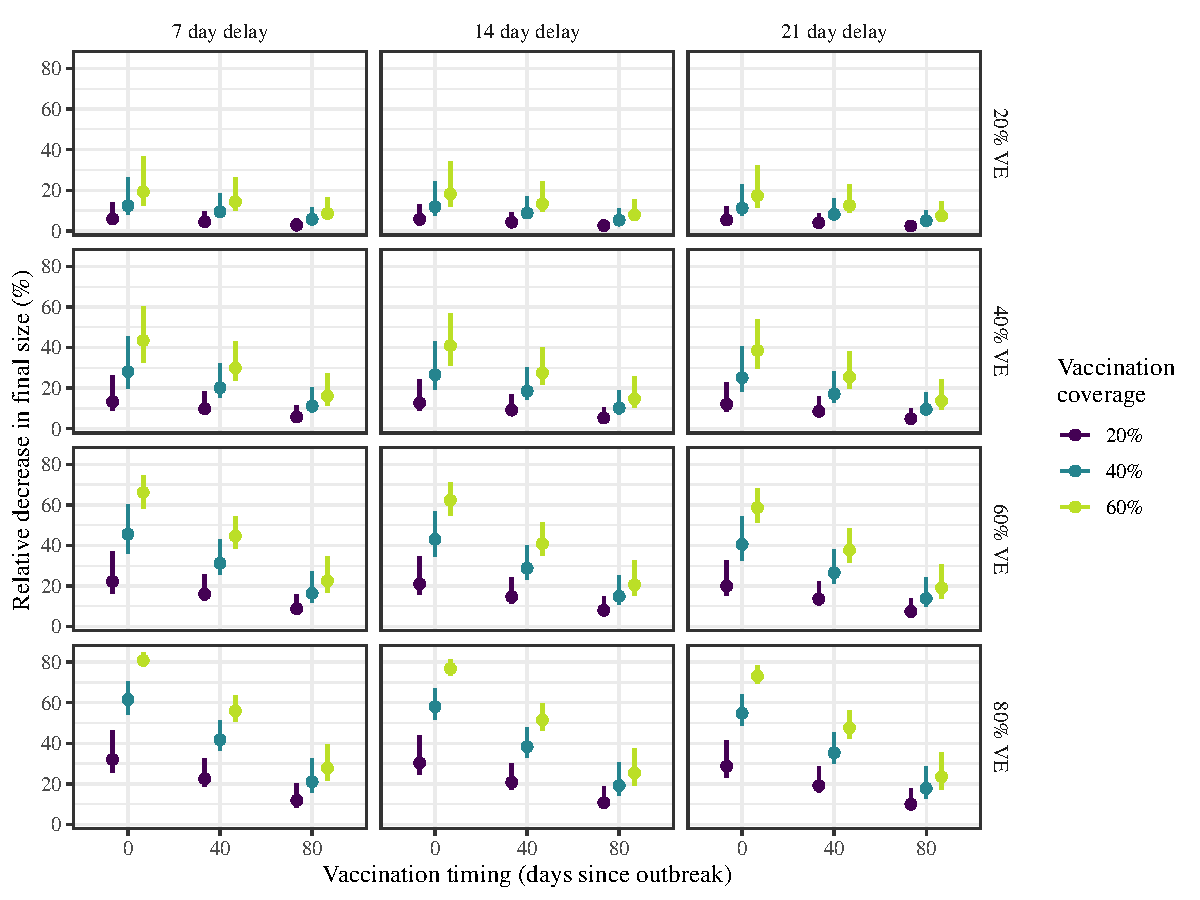
\includegraphics[width=\textwidth]{../figure_stanfit_seirv_final/figure_stanfit_strategy.pdf}
\caption{
\textbf{\DIFaddFL{Impact of different vaccination strategies in reducing transmission.}}
\DIFaddFL{We simulate the model under 108 different vaccination strategies across the posterior distributions.
Then, we evaluate the impact of each vaccination strategy in decreasing the final size of the outbreak, relative to no vaccination scenario.
Points represent median estimates.
Error bars represent 95\% credible intervals.
}}
\label{fig}
\DIFaddendFL \end{figure}


\pagebreak

\bibliography{mumps}

\end{document}
